\documentclass[11pt]{aghdpl}
% \documentclass[en,11pt]{aghdpl}  % praca w języku angielskim
\usepackage[polish]{babel}
%\usepackage[english]{babel}
\usepackage[utf8]{inputenc}
\usepackage[]{algorithm2e}
% dodatkowe pakiety
\usepackage{enumerate}
\usepackage{graphicx}
\usepackage{listings}
\usepackage{mathtools}
\usepackage{hyperref}
\hypersetup{
    colorlinks,
    citecolor=black,
    filecolor=black,
    linkcolor=black,
    urlcolor=black
}
\lstloadlanguages{TeX}

\lstset{
  literate={ą}{{\k{a}}}1
           {ć}{{\'c}}1
           {ę}{{\k{e}}}1
           {ó}{{\'o}}1
           {ń}{{\'n}}1
           {ł}{{\l{}}}1
           {ś}{{\'s}}1
           {ź}{{\'z}}1
           {ż}{{\.z}}1
           {Ą}{{\k{A}}}1
           {Ć}{{\'C}}1
           {Ę}{{\k{E}}}1
           {Ó}{{\'O}}1
           {Ń}{{\'N}}1
           {Ł}{{\L{}}}1
           {Ś}{{\'S}}1
           {Ź}{{\'Z}}1
           {Ż}{{\.Z}}1
}

%---------------------------------------------------------------------------

\author{Stefan Kultys}
\shortauthor{S. Kultys}

\titlePL{Algorytmy przybliżone dla zagadnienia przydziału kwadratowego}
\titleEN{Approximation algorithms for qadratic assignment problem}

\shorttitlePL{Algorytmy przybliżone dla zagadnienia przydziału kwadratowego} % skrócona wersja tytułu jeśli jest bardzo długi
\shorttitleEN{Approximation algorithms for qadratic assignment problem}

\thesistype{Praca dyplomowa magisterska}
%\thesistype{Master of Science Thesis}

\supervisor{dr inż. Wojciech Chmiel}
%\supervisor{Marcin Szpyrka PhD, DSc}

\degreeprogramme{Automatyka i Robotyka}
%\degreeprogramme{Computer Science}

\date{2014}

\department{Katedra Automatyki i Inżynierii Biomedycznej}
%\department{Department of Applied Computer Science}

\faculty{Wydział Elektrotechniki, Automatyki,\protect\\[-1mm] Informatyki i Inżynierii Biomedycznej}
%\faculty{Faculty of Electrical Engineering, Automatics, Computer Science and Biomedical Engineering}

\acknowledgements{Serdeczne podziękowania dla bla bla bla}


\setlength{\cftsecnumwidth}{10mm}

%---------------------------------------------------------------------------
\setcounter{secnumdepth}{4}

\begin{document}

\titlepages
\setcounter{tocdepth}{3}
\tableofcontents
\clearpage

\chapter{Wstęp}
\label{cha:wstep}
Nadejście rewolucji przemysłowej spowodowało powstanie wielkiej liczby firm, przedsiębiorstw, które były dużo większe niż znane wcześniej zakłady rzemieślnicze. Ich rozmiar powodował również rozrost złożoności problemów związanych z organizacją tychże firm. W związku z kompleksowością pojawiły się problemy jak najlepszego przydziału dostępnych zasobów oraz najwłaściwszej organizacji pracy. Zaistniała więc potrzeba stworzenia różnych metod, dzięki którym można by powyższe problemy w jakiś sposób rozwiązać. Ta potrzeba doprowadziła do powstania badań operacyjnych.

Chociaż początki badań operacyjnych faktycznie związane są z rewolucją przemysłową, to jednak pojęcie badań operacyjnych, które znamy obecnie, związane jest z działaniami podejmowanymi przez agencje wojskowe już na początku drugiej wojny światowej. Można by stwierdzić, że pewną ironią losu jest fakt, iż wiele wykorzystywanych dzisiaj odkryć i wynalazków, które bardzo ułatwiają nam  codziennie życie, zostało powołanych do życia w związku z działaniami kojarzącymi się najczęściej z cierpieniem i przemocą. 
Brytyjskie i amerykańskie organizacje wojskowe zatrudniły ogromną liczbę naukowców, by ci wdrożyli naukowe podejście do spraw związanych z efektywnym zbrojeniem się, zarządzaniem zasobami oraz taktycznymi i strategicznymi problemami związanymi z prowadzeniem działań wojennych.

Mówi się, że podjęte wysiłki miały duży wpływ na takie znane wydarzenia jak Bitwa o Anglię, czy też Bitwa o Atlantyk.

Sukces, jaki odniosły badania operacyjne w wojskowości, zachęcił ludzi związanych z przemysłem do zaadaptowania ich również w samym przemyśle. Ożywienie w gospodarce, spowodowane zakończeniem wojny, doprowadziło do wzrostu złożoności działalności firm, a więc badania operacyjne idealnie nadawały się jako narzędzie wspierające organizację i zarządzanie tymi przedsiębiorstwami. 

Niewątpliwie następujący szybki rozwój badań operacyjnych miał swą przyczynę  w tym, że wielu naukowców, którzy parali się nimi podczas wojny, szukając pracy w swojej branży, chętnie zajęło się dalszymi studiami nad badaniami operacyjnymi w dziedzinach związanych nie tylko z wojskowością. Oczywiście nie oznaczało to, że wojsko całkowicie zrezygnowało z badań operacyjnych. Również postęp związany z powstaniem komputerów dał odpowiednie narzędzia do analizy coraz bardziej złożonych problemów. Wiele problemów związanych z podejmowaniem decyzji, wyborem najlepszego rozwiązania można było rozwiązać podpierając się matematycznym modelem. Mając więc problem w sformalizowanej postaci można zaproponować algorytm, który rozwiąże dane zagadnienie. Sam algorytm jako ciąg kolejnych instrukcji, które należy wykonać, by osiągnąć dany cel, bardzo dobrze nadaje się do zaimplementowania i wykonania na komputerze. Coraz szybsze komputery o coraz pojemniejszych pamięciach, a także wykorzystanie technik programowania równoległego i współbieżnego pozwalają na rozwiązywanie coraz bardziej złożonych problemów w rozsądnym czasie. Z czasem więc zaczęły się pojawiać kolejne algorytmy, ale też nowe problemy. Również dokonywane odkrycia naukowe pozwoliły na wykorzystanie występujących w naturze procesów do tworzenia nowatorskich metod rozwiązywania skomplikowanych zagadnień.

Niestety, istnieje wiele problemów, w przypadku których można jedynie powiedzieć, że mają optymalne rozwiązanie, nie da się jednak znaleźć go przy wykorzystaniu obecnie dostępnej technologii. Poprzez oszacowanie złożoności obliczeniowej algorytmów można tylko stwierdzić, że potrzebny czas do znalezienia rozwiązania problemu przy ich wykorzystaniu jest niejednokrotnie dłuższy niż przeciętny czas życia człowieka. Przykładem takiego zagadnienia jest tzw. problem przydziału kwadratowego, polegającego na przydziale pewnej liczby placówek do takiej samej liczby miejsc. Wynika z tego, że dla n placówek możliwe jest w sumie \textit{n!} wszystkich permutacji. Wraz ze wzrostem liczby placówek, które należy przydzielić, ilość możliwych rozwiązań rośnie bardzo szybko. Już dla stosunkowo małej ilości placówek możliwa jest ogromna liczba rozwiązań. Istnieje  więc wiele algorytmów przybliżonych, inaczej nazywanych aproksymacyjnych, które znajdują jedynie przybliżone rozwiązanie postawionego problemu. Nie oznacza to jednak, że zwrócone przez algorytm rozwiązanie nie może być faktycznie optymalne, ale przeważnie nie da się tego sprawdzić.

Jak już zostało to nadmienione wyżej, istnieje wiele algorytmów wykorzystujących analogie do zachowań występujących w przyrodzie. Przykładem są algorytmy genetyczne, których działanie wzorowane jest na ewolucji biologicznej - spośród znalezionych w danym pokoleniu rozwiązań, wybierane są najlepsze z nich (według pewnych ustalonych dla danego problemu kryteriów), traktowane są jako rodzice dla następnego pokolenia, które dziedziczy po rodzicach ich cechy. Wykorzystywane są również różnego rodzaju operatory mutacji, katastrofy itp. 

\section{Cel pracy}
\label{sec:cel}
Celem niniejszej pracy jest dokonanie przeglądu wybranych algorytmów przybliżonych, ich wad i zalet oraz przedstawienie ich wykorzystania w kontekście problemu przydziału kwadratowego. Następnie, przy użyciu specjalnie napisanej na potrzeby pracy aplikacji, która rozwiązuje problem przydziału kwadratowego, należy zaprezentować rezultaty przeprowadzonych eksperymentów oraz opisać zastosowane scenariusze testowe i dokonać analizy otrzymanych wyników.

\section{Zawartość pracy}
\label{sec:zawartosc}
Rozdział nr 2 zawiera opis problemu przydziału kwadratowego, obszar jego zastosowań i jego model matematyczny.

W rozdziale trzecim zostały przedstawione wybrane algorytmy aproksymacyjne, geneza ich powstania oraz wybrane sposoby ich wykorzystania w celu rozwiązania problemu przydziału kwadratowego.

Rozdział czwarty poświęcony jest idei kwantowych algorytmów ewolucyjnych, a także opisano w nim wybrany algorytm kwantowy NPQGA, który został zaimplementowany w aplikacji będącej jednym z celów niniejszej pracy. Wprowadzone zmiany i modyfikacje we wspomnianym algorytmie są tematem kolejnego, piątego rozdziału pracy.

Następny, szósty rozdział zawiera opis utworzonej aplikacji, informacje o działaniu algorytmu i obsłudze programu.

Rozdział siódmy omawia metodykę eksperymentów przeprowadzanych przy wykorzystaniu napisanej aplikacji. Zawarte w nim są opisy wybranych instancji testowych, a także przedstawione są scenariusze testowe.

Rozdział ósmy  poświęcony jest faktycznie przeprowadzonym eksperymentom, zawiera informacje o tym, jakie ustawienia parametrów algorytmu były testowane i porównywane dla wybranych instancji testowych.

W kolejnym rozdziale zostały przedstawione rezultaty opisanych w poprzednim rozdziale testów, zawarte zostały wykresy obrazujące działanie algorytmów dla różnych nastaw oraz różne statystyki dające obraz o tym, jaki wpływ na rezultaty mają zmiany w ustawieniach konkretnych parametrów.

Rozdział dziesiąty skupia się na analizie rezultatów uzyskanych z przeprowadzonych testów. Opisane są wnioski dotyczące poszczególnych eksperymentów.

Ostatni, jedenasty rozdział poświęcony jest ogólnym wnioskom dotyczącym tematyki całej pracy oraz jej podsumowaniu.
\chapter{Zagadnienie przydziału kwadratowego}
\label{cha:qap}

\section{Opis problemu}
\label{sec:opis}
Zagadnienie przydział kwadratowego (Qadratic Assignment Problem - QAP) jest jednym najtrudniejszych problemów optymalizacji kombinatorycznej. Należy on klasy problemów NP - trudnych i dla rozmiarów o wartości większej niż 30 wymagane jest stosowanie algorytmów przybliżonych w celu jego rozwiązania. Zagadnienia przydziału kwadratowego zostało przedstawione przez Koopmansa i Beckmanna w roku 1957. Problem ten jest matematycznym modelem sytuacji, w której chcemy przydzielić pewną ilość placówek do takiej samej ilości lokalizacji (miejsc) znając przy tym odległości pomiędzy danymi lokalizacjami oraz przepływu miedzy placówkami. Przydziału tego należy dokonać minimalizując koszt tej operacji, który jest proporcjonalny do przepływu pomiędzy placówkami pomnożonego przez odległość między miejscami, do których te placówki zostały przydzielone. Z racji, iż trudność rozwiązania tego problemu jest duża oraz, że modeluje on wiele faktycznych zagadnień, wielu autorów poświęciło mu dużo uwagi, przez co znaleźć można wiele różnych publikacji traktujących o problemie QAP.

\section{Obszary zastosowań}
\label{sec:zastosowanie}
Przy pomocy problemu przydziału kwadratowego można modelować wiele różnych zagadnień, które występują wokoło. Do dziedzin,w których zagadnienie QAP znajduje zastosowanie należą m. in:
\begin{itemize}
\item ekonomia,
\item informatyka,
\item elektronika, np. projektowanie układów elektroniki,
\item logistyka, np. lokalizacja współpracujących ze sobą fabryk, zakładów produkcyjnych, oddziałów w szpitalach,
\item mechanika - wyważanie turbin w silnikach odrzutowych.
\end{itemize}
\chapter{Algorytmy przybliżone}
\label{cha:algorytmy}

Złożoność otaczającego nas świata powoduje, że bardzo często występujące problemy, które chcielibyśmy rozwikłać są w rzeczywistości bardzo trudne do rozwiązania. Dotyczy to praktycznie każdej sfery ludzkiego życia. W wielu sytuacjach natura problemu nie pozwala na zastosowanie metod matematycznych, jednakże nawet w przypadku takich trudności, w których matematyka przychodzi z pomocą, można stwierdzić jedynie, że problem ma rozwiązanie i to nawet najlepsze z możliwych, optymalne, lecz znalezienie go jest praktycznie niewykonalne. Używając języka naukowego, wiele z tych problemów można nazwać NP-trudnymi. Złożoność obliczeniowa algorytmów pozwalających na rozwiązanie ich jest zbyt duża, by w ogóle warto było je stosować. Pojawia się więc potrzeba zastosowania czegoś, co pozwoli na znalezienie rozwiązania dobrego, przybliżającego chociaż rozwiązanie optymalne. I faktycznie jest grupa algorytmów, które pozwalają na uzyskanie takiego efektu. Są to algorytmy przybliżone, inaczej zwane aproksymującymi.

W przeciwieństwie do problemów optymalizacji, których rozwiązanie jest możliwe do znalezienia w czasie wielomianowym, problemy NP-trudne nie dają \" punktu wyjścia\" do znalezienia rozwiązania optymalnego. Jednakże, niejednokrotnie istnieje \"punkt wyjścia \", który pozwala na dojście do rozwiązania znajdującego się w pobliżu rozwiązania najlepszego. W tym sensie algorytmy przybliżone podobne są do algorytmów dokładnych: również polegają na uchwyceniu istoty problemu i następnie na znalezieniu algorytmu, która pozwoli na wykorzystanie jej.

Ogromna ilość problemów, dla których nie jesteśmy w stanie znaleźć rozwiązania optymalnego, przyczyniła się do powstania wielu algorytmów aproksymacyjnych.  Przy tworzeniu algorytmów dąży się do tego, by działały one jak najszybciej. W przypadku rozwiązywania przy ich użyciu problemów niejednokrotnie czas ich działania jest dosyć długi. Jednakże, pozwalają one na znalezienie dobrego rozwiązania w sytuacji, gdy użycie algorytmów dokładnych nie pozwoliłoby uzyskać rozwiązania w ogóle.

Ciekawą rzeczą związaną z algorytmami przybliżonymi jest fakt, że wiele z nich powstało na podstawie obserwacji zjawisk występujących w przyrodzie.

Poniżej zostaną przedstawione kilka algorytmów aproksymujących, zostaną przedstawione podstawowe informacje na ich temat, opisany schemat ich działania, a także to, w jaki sposób przy ich pomocy można by próbować rozwiązać problem QAP.
\section{Particle Swarm Optimization}
\label{sec:PSO}
\subsection{Geneza i opis algorytmu}
Algorytm Particle Swarm Optimization (PSO), czyli algorytm optymalizacji rojem cząstek, po raz pierwszy został przedstawiony w pracy Jamesa Kennedy'ego i Russella Eberharta w 1995 roku, jako metoda optymalizacji nieliniowych funkcji ciągłych. Metoda powstała w oparciu o przeprowadzane symulacje uproszczonych modeli zachowań społecznych. Inspiracją dla autorów były przeprowadzane przez naukowców komputerowe symulacje zachowań stad ptaków czy ławic ryb.

Zachowania stad ptaków zawsze interesowały naukowców. Chcieli oni dociec w jaki sposób ptaki potrafią, latając w licznych stadach, lecieć w sposób synchroniczny, często zmieniając kierunek lotu czy też błyskawicznie się przegrupowując. Z czasem powstawały różnego rodzaju modele tychże zachowań, programy pozwalające na symulowanie ich. Również ciekawą rzeczą był fakt, że ptaki potrafią znaleźć sobie pożywienie, ominąć zagrożenie, mimo że nie posiadają początkowo wiedzy na ten temat. Pojawiły się tezy, że potrafią one wykorzystać zdobytą wiedzę przez inne osobniki, czy tez poprzednie pokolenia. Dążenie do znalezienia pokarmu, próby unikania sytuacji niebezpiecznych czy drapieżników są czynnikami decydującymi o poprawie \"sytuacji życiowej\" ptaków. Jest to swego rodzaju optymalizacja dokonywana samoistnie przez naturę. Analiza tych zachowań stała się punktem wyjścia do tworzenia algorytmów pozwalających na rozwiązywanie wielu trudnych problemów.

Algorytm PSO w pewien sposób przypomina wspomniane wcześniej symulacje, lecz zawiera też parę istotnych różnic. W klasycznej wersji, algorytm zawiera rój cząstek poruszających się w wielowymiarowej przestrzeni, który inicjowany jest w sposób losowy. Cząstki te reprezentują rozwiązania problemu i scharakteryzowane są swoją prędkością i położeniem. Ruch cząstek w kolejnych iteracjach ma na celu przeszukiwanie przestrzeni rozwiązań. Każda z cząstek zapamiętuje znalezioną przez siebie dotychczas najlepszą pozycję. W oparciu o te pozycje, w każdej iteracji cząstki mają aktualizowaną swoją prędkość i położenie.

Algorytm PSO posiada wiele zalet. Przede wszystkim jest bardzo prosty i wydajny, oraz pozwala na optymalizację wielu różnych funkcji. Aktualizacja prędkości i położenia cząstek wymaga jedynie podstawowych operacji matematycznych. Algorytm nie wymaga również zapamiętywania dużej ilości danych, dlatego jest wydajny z punktu widzenia szybkości działania i nie wymaga wielu zasobów pamięci. Ważną cechą jest również to, że jest on bardzo odporny na wpadnięcie do minimum lokalnego.

\subsection{Model matematyczny algorytmu}
Model matematyczny algorytmu PSO może być przedstawiony w następujący sposób:
\textit{Mamy dany rój cząstek, który składa się z n cząstek. Każda z nich porusza się w d-wymiarowej przestrzeni. Każda z cząstek opisana jest przez dwa wektory:}

\begin{itemize}
\item\textit{wektor położenia:}
\newline
\begin{equation}
x_i = [x_{i1},x_{i2},...,x_{id}]
\end{equation}
\newline
\item\textit{wektor prędkości:}
\newline
\begin{equation}
v_i = [v_{i1},v_{i2},...,v_{id}]
\end{equation}
\newline
\end{itemize}

\textit{Ponadto, każda z cząstek zapamiętuje znalezioną przez siebie najlepszą dotychczas pozycję w wektorze:}
\newline
\begin{equation}
x_i^b=[x_{i1}^b,x_{i2}^b,...,x_{id}^b]
\end{equation} 
\newline
\textit{Zapamiętywana jest również w wektorze $x^*$ najlepsza dotychczas pozycja w ogóle znaleziona przez wszystkie cząstki w roju.}

\textit{Wartości prędkości i położenia w każdej iteracji algorytmu aktualizowane są odpowiednio według poniższych wzorów[odniesienie]:}
\newline
\begin{equation}
v_{ij}(t)=w \cdot v_{ij}(t-1)+c_1\cdot r_1 \cdot (x_{ij}^b(t-1)-x_{ij}(t-1))+c_2 \cdot r_2 \cdot (x_j^*(t-1)-x_{ij}(t-1))
\end{equation}
\newline
\begin{equation}
x_{ij}(t)=x_{ij}(t-1)+v_{ij}(t)
\end{equation}
\newline
\textit{gdzie liczby $r_1$ i $r_2$ są wybierane losowo z przedziału $[0,1]$, natomiast współczynniki $c_1$ i $c_2$ odpowiadają za to, w jakim stopniu do aktualizacji prędkości brane są pod uwagę najlepsze znalezione dotychczas położenia każdej z cząstek z osobna i najlepsze położenie w ogóle. Parametr $w$ określa bezwładność cząstek i z czasem maleje liniowo do $0$.}

\subsection{Pseudokod dla algorytmu PSO}
Poniżej znajduje się pseudokod, który opisuje jak krok po kroku działa algorytm optymalizacji rojem cząstek:
\newpage
\begin{algorithm}[H]
	Wczytaj rozmiar roju n, wymiar d, ilość iteracji t i inne parametry\;
 	\While{nie wystąpił warunek stopu}
 	{
 		$t\leftarrow t+1$\;
  		\For{$i\leftarrow 1$ \KwTo $n$}
  		{
  			Policz dopasowanie cząstki $x_i$\;
  			\If{$x_i$ jest lepsza niż $x_i^b$}
  			{
  				$x_i^b \leftarrow x_i$
  			}
  			\If{$x_i^b$ jest lepsza niż $x^*$}
  			{
  				$x^* \leftarrow x_i^b$
  			}
  		}
  		\For{$i\leftarrow 1$ \KwTo $n$}
  		{
  			\For{$j\leftarrow 1$ \KwTo $d$}
  			{
  				Zaktualizuj prędkość $v_{ij}$\;
  				Zaktualizuj położenie $x_{ij}$\;
  			}
  		}
 	}
 	\caption{Algorytm PSO}
\end{algorithm}

\subsection{Zastosowanie algorytmu PSO dla problemu QAP}
Aby było możliwe zastosowanie algorytmu PSO do rozwiązania problemu przydziału kwadratowego, należy odpowiednio ująć problem QAP, by dało się go wpasować w model algorytmu. Przede wszystkim rozwiązaniami zagadnienia przydziału kwadratowego są permutacje, czyli jest to problem dyskretny. Pozycje cząstek w algorytmie PSO mogą zmieniać się w sposób ciągły, położenie nie musi być określone współrzędnymi całkowitymi. Również w permutacji liczby nie mogą się powtarzać. Natomiast nie stoi nic na przeszkodzie, by zwrócona przez algorytm pozycja cząstki była opisana w każdym kierunku przez współrzędne o tej samej wartości. Proste mapowanie: wartość położenia w $i-tym$ kierunku określa przydzielenie do $i-tej$ lokalizacji obiektu o tejże wartości może powodować, że dany obiekt będzie przydzielony wielokrotnie.
\section{Algorytm Tabu Search}
\label{sec:TS}
\subsection{Geneza i opis algorytmu}
Algorytm Tabu Search został zaproponowany przez Freda Glovera w roku 1986. Jest to metaheurystyka pozwalająca innym metodom optymalizacji unikać sytuacji, w których te wpadają w minima lokalne. Dzięki metodzie tabu search udało się znaleźć optymalne lub prawie optymalne rozwiązania dla bardzo wielu problemów optymalizacji takich jak szeregowanie zadań, problem przydziału kwadratowego, rozpoznawanie charakteru, kolorowanie grafów.

Słowo tabu kojarzone jest przede wszystkim z czymś zakazanym, najczęściej na tle kulturowym. W przypadku algorytmu należy je rozumieć bardziej jako ograniczenie. W ogólności algorytm tabu search polega na zabranianiu wykonywania danej operacji modyfikującej rozwiązanie zwanej ruchem. Ruch jest funkcją, która transformuje dane rozwiązanie w inne, w przypadku permutacji może to być zamiana miejscami dwóch liczb. W danym momencie możliwy jest pewien podzbiór rozwiązań, w które inne może być przetransformowane. Z dostępnych ruchów wybierany jest ten, który powoduje polepszenie rozwiązania i ostatnio wykonany ruch dodawany jest do tablicy ruchów zabronionych na pewną określoną liczbę iteracji algorytmu. Mechanizm ten pozwalaj na wyjście z minimum lokalnego i pozwala uniknąć ruchów cyklicznych. Jednakże w pewnych określanych sytuacjach możliwe jest wykonanie ruchu zabronionego. Zdefiniowana jest specjalna funkcja, zwana funkcją aspiracji, która pozwala obliczyć, czy zabroniony ruch będzie jednak opłacalny.

Algorytm zatrzymuje się, gdy spełniony jest jeden z warunków zatrzymania. Takimi warunkami mogą być wykonanie z góry założonej iteracji algorytmu czy też wykonaniu ustalonej liczby ruchów, które nie prowadzą do dalszej poprawy rozwiązania.

\subsection{Pseudokod algorytmu Tabu Search}
\begin{algorithm}[H]
	Inicjalizuj pierwsze rozwiązanie x\;
	Inicjalizuj rozwiązanie najlepsze $x^b$: $x^b \leftarrow x$\;
 	\While{nie wystąpił warunek stopu}
 	{
 		Przygotuj listę możliwych ruchów dla obecnego rozwiązania\;
 		Wybierz najlepszy możliwy ruch z uwzględnieniem tablicy tabu i kryterium aspiracji\;
 		Przypisz otrzymane w ruchu rozwiązanie do rozwiązania aktualnego x\;
 		\If{rozwiązanie x jest lepsze od $x^b$}
 		{
 			$x^b \leftarrow x$
 		} 		
 		Zaktualizuj tablicę tabu i kryterium aspiracji\;		
 	}
 	\caption{Algorytm Tabu Search}
\end{algorithm}

\subsection{Zastosowanie algorytmu Tabu Search dla problemu QAP}
Rozwiązaniami problemu przydziału kwadratowego są permutacje określające przydział placówek do lokalizacji. Należy więc, mając dane aktualne rozwiązanie problemu QAP, określić w jaki sposób będzie wykonywany ruch w kolejnych iteracjach działania algorytmu. Zmiana aktualnego rozwiązania musi odbyć się w sposób, który nie spowoduje, że do danej lokalizacji zostanie przypisany więcej niż jeden obiekt, jak również któryś z obiektów nie zostanie desygnowany do żadnego z miejsc. W przeciwieństwie do, przykładowo, algorytmu PSO, strategia Tabu Search pozwala na przeszukiwanie przestrzeni rozwiązań w sposób dosyć prosty. Istnieje wiele metod dokonywania ruchów w przypadku, gdy rozwiązanie jest permutacją. Najczęściej spotykanym w literaturze jest sposób polegający na zamianie miejscem dwóch elementów permutacji. Wynika stąd, że dla permutacji o długości $n$ istnieje $n\choose 2$ kombinacji takiego wyboru. Wykonane ruchu zapisywane są w tablicy tabu i trzymane są w niej przez określoną liczbę iteracji algorytmu. Poniżej znajduje się przykładowa tablica:
\begin{figure}[h]
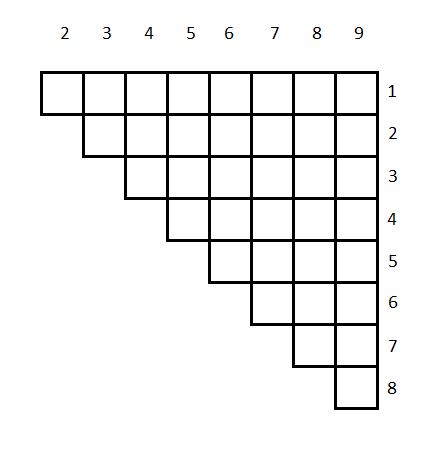
\includegraphics[scale=0.8]{tabu}
\end{figure}

W powyższej tablicy w komórce o indeksie $(i,j)$ wpisuje się liczbę iteracji algorytmu, podczas których zamiana obiektów o wartości (nie indeksie) nie można zamienić miejscami. Po każdej iteracji liczba ta jest zmniejsza o $1$. Wpis dodawany jest, gdy nastąpiła zamiana miejscami obiektów o wartościach $i$ i $j$.

Innymi metodami pozwalającymi na wykonanie ruchu w algorytmie TS są przykładowo wstawienie jednego z elementów permutacji w inne miejsce i przesunięcie pozostałych elementów, czy też inwersja wybranej grupy elementów permutacji o określonej szerokości.
\section{Algorytm mrówkowy}
\label{sec:mrowka}
\subsection{Geneza i opis algorytmu}
Algorytm mrówkowy (Ant Algoirthm) został stworzony przez Marco Dorigo, jak metoda rozwiązywania trudnych problemów optymalizacji jakimi są przykładowo problem komiwojażera (TSP, Travelling Salesman Problem) czy problem przydziału kwadratowego QAP. Inspiracją do powstania algorytmu była obserwacja faktycznych, istniejących w naturze, rojów mrówek. Uwagę naukowców przykuło to, że mrówki, które same są dosyć prostymi stworzeniami, działając w grupie potrafią osiągnąć wysoki poziom organizacji, żyją w zhierarchiwizowanym społeczeństwie. Również ciekawą cechą w zachowaniu mrówek jest to, że nastawione są bardziej na przeżycie całej społeczności niż pojedynczego osobnika. Posiadają one także niespotykane umiejętności pozwalające im na znajdywanie najkrótszej drogi pomiędzy mrowiskiem a     miejscem, w którym znajduje się pożywienie.

Ważnym czynnikiem pozwalającym na znajdywanie najkrótszej ścieżki do źródła pokarmu oraz zapamiętywania tejże drogi są substancje chemiczne wydzielana przez mrówki, zwane feromonami. Insekty te mają zdolność wyczuwania feromonów i dzięki temu najprawdopodobniej potrafią wybrać drogę, dla której stężenie feromonów jest największe. Pozwala to również innym osobnikom, na wykorzystanie informacji o lokacji pożywienia zdobytej przez inne mrówki.

Można w związku z powyższym metaforycznie stwierdzić, że mrówki posiadają zdolność wychodzenia z minimów lokalnych i wybierają minimum globalne.

\subsection{Model matematyczny algorytmu}
\subsection{Zastosowanie algorytmu mrówkowego dla problemu QAP}

\section{Algorytmy ewolucyjne}
\label{sec:AE}

Algorytmy ewolucyjne są najogólniej rzecz biorąc algorytmy optymalizacji, które bazują na stopniowym polepszaniu pewnej populacji rozwiązań danego problemu. Z powodzeniem są stosowane od wielu lat do rozwiązywania wielu zarówno praktycznych jak i teoretycznych problemów. Istnieje wiele różnorodnych implementacji algorytmów ewolucyjnych. Należą do nich między innymi[evolutionary PDF]:
\begin{itemize}
\item algorytmy genetyczne, stworzone przez Johna Henry'ego Hollanda,
\item strategie ewolucyjne,opracowane przez Ingo Rechenberga oraz Hansa Paul Schwefela,
\item programowanie ewolucyjne stworzone przez Lawrence'a Fogela.
\end{itemize}

Algorytmy ewolucyjne posiadają wiele cech, które odróżniają je od innych metod optymalizacji. Przede wszystkim zmianom poddawana jest zakodowana w łańcuchu znaków postać problemu , a nie jego parametry bezpośrednio i wykorzystywane jest doświadczenie poprzednich pokoleń. Łańcuch ten ma ustaloną długość i korzysta ze znaków ze skończonego alfabetu. Jak już zostało to wspomniane wcześniej, przetwarzana jest też pewna populacja rozwiązań, nie jedno. By ocenić dane rozwiązanie potrzebna jest jedynie funkcja celu, bądź też coś, co pozwoli porównać dwa rozwiązania i wyłonić lepsze z nich. Kolejnym elementem, który cechuje algorytmy ewolucyjne jest fakt, że stosowane są w nich niedeterministyczne, probabilistyczne reguły wyboru.

Algorytmy genetyczne są chyba najczęściej stosowanymi i najbardziej znanymi implementacjami algorytmów ewolucyjnych. Często, choć niepoprawnie, terminy \textit{algorytmy ewolucyjne} oraz \textit{algorytmy genetyczne} stosowane są zamiennie. Z powodu ich popularności, dalsza część rozdziału będzie poświęcona tejże podgrupie algorytmów ewolucyjnych.

\subsection{Geneza i opis algorytmów genetycznych}
Algorytmy genetyczne zostały opracowane, jak już zostało to wspomniane, przez Johna Hollanda przy pomocy jego kolegów i studentów związanych z Uniwersytetem Michigan. Celami, które im przyświecały podczas tworzenia algorytmów były chęć opisania oraz wyjaśnienie istoty zjawisk zachodzących w świecie przyrody, dzięki którym możliwa jet adaptacja do różnych warunków, a także utworzenie oprogramowania mogącego symulować mechanizmy obecne w systemach biologicznych. Ważną cechą rzeczywistych systemów biologicznych jest odporność tych systemów. Potrafią one szybko zaadaptować się do zmieniających się warunków ich otaczających, posiadają duże zdolności regeneracyjne. Niewątpliwie są to cechy pożądane także przy projektowaniu różnego rodzaju systemów: inżynierskich, ekonomicznych. Skoro algorytmy genetyczne pojawiły się w oparciu o symulacje zjawisko zachodzących w naturze, może pojawić się pytanie czy one same posiadają podobne zdolności. Odpowiedź na nie podał Holland w roku 1975 udowadniając, że algorytmy genetyczne są odporną metodą poszukiwania rozwiązań nawet w skomplikowanych przestrzeniach. Inną ważną zaletą algorytmów genetycznych jest to, że stosowanie ich nie wymaga spełniania założeń dotyczących przestrzeni poszukiwań jakimi są przykładowo ciągłość czy różniczkowalność. Dzięki stosowaniu probabilistycznych technik wyboru, a także dzięki przetwarzaniu całej populacji rozwiązań, w przeciwieństwie do wielu innych analitycznych metod optymalizacji, zmniejszona znacznie jest szansa na zatrzymanie się w ekstremum lokalnym. W tym sensie metody analityczne przejawiają swój brak odporności.
Jednakże, z faktu, iż algorytm genetyczny jest metodą przybliżoną, w przypadku optymalizowania wielu problemów nie jest możliwe stwierdzenie, czy znalezione rozwiązanie, zwrócone przez algorytm jest optymalne i jak daleko znajduje się od optimum. Nie można również zagwarantować, że start algorytmu przy pewnych początkowych ustawieniach zawsze zwróci ten sam rezultat.

W klasycznej, najprostszej wersji, algorytm genetycznych składa się z kilku podstawowych operacji. Mając wygenerowaną losowo populację początkową uruchamiamy algorytm na określoną liczbę operacji. W każdej iteracji dokonujemy oceny każdego z rozwiązań w populacji i w oparciu o ich wartość dopasowania rozwiązań dokonujemy selekcji osobników, na których będą wykonane operacje krzyżowania oraz mutacji. W zależności od postaci rozwiązania, a także od metody jego kodowania, operatory genetyczne mogą działać w różnoraki sposób. W ogólnym przypadki, krzyżowanie polega na wymianie informacji pomiędzy osobnikami wybranymi na drodze selekcji, a mutacja na losowej zmianie wybranego rozwiązania, mogącej zmienić dane rozwiązanie na lepsze bądź gorsze. Teoretycznie z każdą iteracją, ogólne dopasowanie całego pokolenia powinno się polepszać. Ogólną ideą algorytmu jest przetrwanie najsilniejszych i eliminacja słabszych.

\subsection{Operatory selekcji}
Już sam sposób doboru osobników, które posłużą za podstawę dla kolejnego pokolenia, ma kluczowe znaczenie. Istnieje wiele sposobów wyboru rozwiązań. Do takich metod można zaliczyć między innymi:
\begin{itemize}
\item metoda ruletki,
\item metoda rankingowa,
\item metoda turniejowa.
\end{itemize}

Metoda ruletki polega na "kręceniu" wirtualną ruletką, na której każde z rozwiązań z aktualnej populacji ma wyznaczony swój wycinek koła. Szerokość wycinka zależy od dopasowania danego rozwiązania. Dla każdego rozwiązania jest liczona wartość funkcji dopasowania, a także liczona jest suma wszystkich wartości dopasowania. Stosunek wartości dopasowania danego osobnika do sumy wszystkich dopasowań wyznacza szerokość wycinka ruletki dla danego rozwiązania. Metoda ta faworyzuje osobniki lepsze, nie pozbawiając jednak szansy wyboru tych gorszych. Jednak może to prowadzić w sytuacji, gdy jedno z rozwiązań jest wyraźnie lepsze od pozostałych, że osobniki wybrane do krzyżowania będą się składać głownie z tego jednego.

Metoda bazująca na rankingu rozwiązań nieco zmniejsza rolę dopasowania danego rozwiązania w kontekście jego szans do bycia wybranym na rodzica. W tej metodzie rozwiązania są szeregowane według swojego dopasowania, a o prawdopodobieństwie wyboru decyduje pozycja w rankingu. W oparciu o ranking definiuje się funkcję, która określa ile kopii danego rozwiązania jest brane pod uwagę. W tym sposobie dysproporcje między prawdopodobieństwami wyboru rozwiązań są mniejsze w stosunku do metody ruletkowej.

Metoda turniejowa polega na losowym wyborze dwóch rozwiązań z populacji i rozwiązanie lepsze z tej pary jest brane pod uwagę w dalszych operacjach. Rozwiązania lepsze mają taką samą szansę bycia wybranym do porównania co te słabsze, lecz i tak w przypadku pojedynku, to one wygrają.

Należy również wspomnieć, że funkcja dopasowania powinna zwracać liczby nieujemne i dla rozwiązania lepszego jego wartość dopasowania powinna być większa, niż dla gorszego. Nie zawsze da się taką informacje uzyskać bezpośrednio z funkcji celu. Znana jest własność dualności zadań minimalizacji kosztu i maksymalizacji zysku, lecz w przypadku funkcji przystosowania, zwracana wartość zawsze musi być nieujemna. Z tego powodu należy dokonać przekształcenia funkcji celu w funkcję dopasowania. Najczęściej  dokonywane to jest poprzez odejmowanie wartości funkcji celu od pewnej liczby. Jeśli taka różnica jest ujemna, zwracamy 0. Wartość tej liczby może być ustalona w wieloraki sposób. Przykładowo, może to być z góry ustalona liczba, może też być modyfikowana wraz z kolejnymi iteracjami algorytmu, np. może przyjąć wartość największej znalezionej do tej pory wartości funkcji celu.

\subsection{Operatory krzyżowania}
Celem operatorów krzyżowania, zwanych inaczej mieszania, jest spowodowanie wymiany informacji pomiędzy wybranymi rozwiązaniami i utworzenie na tej podstawie kolejnych. Mając wyselekcjonowaną populacje rozwiązań, łączymy w pary osobniki i dokonujemy ich krzyżowania. To w jaki sposób zostanie to wykonane zależy od postaci rozwiązania. Istnieje wiele różnych metod krzyżowania. Inne są wykorzystywane dla rozwiązań kodowanych w sposób binarny, inne dla kodów wykorzystujących liczby rzeczywiste itp. Do najbardziej znanych metod krzyżowania należą:
\begin{itemize}
\item krzyżowanie jednopunktowe,
\item krzyżowanie wielopunktowe,
\item krzyżowanie z częściowym odwzorowaniem PMX,
\item krzyżowanie cykliczne CX,
\item krzyżowanie z zachowaniem porządku OX.
\end{itemize}

Trzy ostatnie z wymienionych operatorów dotyczy rozwiązań będących permutacjami i ich użycie pozwala na zachowanie tej postaci po dokonaniu krzyżowania. Operatory jednopunktowy i wielopunktowy powodują wymianę pomiędzy osobnikami fragmentów kodu pomiędzy wylosowanymi punktami. Operacja krzyżowania wykonywana jest z pewnym określonym jako parametr algorytmu prawdopodobieństwem. Dla każdego z rozwiązań, wybranych na drodze selekcji, losowane jest czy będzie brane pod uwagę w dalszych działaniach. W zależności od przyjętych założeń, może zaistnieć potrzeba doboru dodatkowych rozwiązań w przypadku, gdy jest ich niewystarczająca ilość, by móc dokonać operacji krzyżowania.

\subsection{Operatory mutacji}
Operacja mutacji jest losową zmianą dokonywaną na rozwiązaniach wzorowaną na mutacjach występujących faktycznie w przyrodzie. Jest ona błądzeniem przypadkowych w przestrzeni ciągów kodowych[goldberg]. Operator mutacji pozwala na przywrócenie utraconych ważnych informacji w kodzie rozwiązania, bądź na uzyskanie dobrych (lub złych) cech w rozwiązaniu, których często nie dałoby się otrzymać na drodze krzyżowania. Z racji iż prawdopodobieństwo wystąpienia mutacji jest wielokrotne mniejsze niż wystąpienie krzyżowania, operacja ta odgrywa drugorzędną rolę w działaniu algorytmu, choć niejednokrotnie pozwala na uzyskanie zaskakujących rezultatów.

W przypadku binarnej postaci kodu rozwiązań operacja mutacji najczęściej polega na zamianie wartości bit z $0$ na $1$ i na odwrót. W innych przypadkach mutacja polega na zmianie wybranego elementu na inny dopuszczalny. W sytuacji, gdy rozwiązaniem jest permutacja, należy zadbać, by operator mutacji pozostawiał rozwiązanie w poprawnej postaci. Mutacja w takim przypadku może polegać przykładowo na zamianie miejscami dwóch elementów, czy też na inwersji pewnego fragmentu kodu. 

\subsection{Schemat działania algorytmu genetycznego}
Poniżej znajduje się pseudokod dla klasycznej wersji algorytmu genetycznego:
\begin{algorithm}[H]
	Inicjalizuj populację początkową\;
 	\While{nie wystąpił warunek stopu}
 	{
 		Dokonaj selekcji rozwiązań będącej podstawą dla nowego pokolenia;\
 		Dokonaj operacji krzyżowania na wybranych osobnikach\;
 		Dokonaj operacji mutacji na osobnikach otrzymanych na drodze krzyżowania\;
 		Zaktualizuj populację w oparciu o otrzymane rozwiązania w wyniku działania operatorów genetycznych
 	}
 	\caption{Algorytm genetyczny}
\end{algorithm}
\subsection{Zastosowanie algorytmu PSO dla problemu QAP}
Algorytm genetyczny można w łatwy sposób zaimplementować dla problemu QAP. Postać rozwiązania problemu przydziału kwadratowego to permutacja. Należy więc na każdym etapie działania algorytmu dokonywać zmian w taki sposób, by zwracane w kolejnych iteracjach populacje rozwiązań były populacjami permutacji. Wyżej zostały wymieniowe metody krzyżowania, takie jak operatory OX, PMX, CX, i mutacji, które mogą być stosowane dla rozwiązań permutacyjnych.
Optymalizacja problemu QAP polega na minimalizacji kosztu przydziału obiektów do lokalizacji. Z tego powodu funkcja celu (wzór) nie nadaje się wprost do oceny przystosowania osobników. Funkcję dopasowania można więc uzyskać z funkcji celu poprzez odejmowanie wartości funkcji celu od pewnej liczby, którą może być największa znaleziona dotychczas wartość funkcji celu, czy też najgorsza wartość dopasowania w ostatniej iteracji itp.
\chapter{Zastosowanie algorytmu quantum EA dla zagadnienia QAP}
\label{cha:qap_ea}
Sposób w jaki działają algorytmy ewolucyjne, ich otwarty schemat działania, skłania do tworzenia wielu modyfikacji. Przykładowo, w kontekście algorytmów genetycznych, zmianom mogą podlegać operatory krzyżowania, mutacji, sposób kodowania rozwiązania. Można dodawać też nowe operatory o działaniu nieobjętym przez tradycyjne operatory. Z tego powodu, na przestrzeni lat, pojawia się wiele publikacji na temat algorytmów ewolucyjnych i nowych sposób podejścia do tego tematu. W jednej z takich publikacji \cite{NPQGA}, autorzy Jinwei Gu, Xingsheng Gu i Manzhan Gu zaproponowali algorytm o nazwie \textit{,,a novel parallel quantum genetic algorithm'' - NPQGA} i przedstawili jego wykorzystanie dla problemu szeregowania zadań.  Algorytm ten należy do grupy tak zwanych kwantowych algorytmów ewolucyjnych i nadaje się także dla innych zastosowań do jakich należy na przykład problem QAP.

\section{Opis algorytmu}
Główną cechą kwantowych algorytmów ewolucyjnych jest zastosowanie w nich bitów kwantowych - kubitów. Wykorzystywane są one do reprezentacji rozwiązań algorytmów. Kubit w danym momencie może reprezentować teoretycznie nieskończenie wiele stanów będących superpozycją stanu $0$ i $1$. Obserwacja bitu kwantowego pozwala dopiero na jednoznaczną ocenę jego stanu. Stan kubitu może być reprezentowany przez równanie:
\newline
\begin{equation}
|\psi\rangle=\alpha|0\rangle+\beta|1\rangle
\end{equation}
\newline
gdzie $|\alpha|^2$ jest prawdopodobieństwem, że kubit znajduje się w stanie $0$, oraz $|\beta|^2$ jest prawdopodobieństwem, że kubit jest w stanie $1$. $\alpha$ i $\beta$ są liczbami zespolonymi. Obie liczby są znormalizowane, co znaczy, że:
\newline
\begin{equation}
|\alpha|^2+|\beta|^2=1
\end{equation}
\newline 

Kubit jest więc najmniejszą jednostką informacji w tych algorytmach i jest reprezentowany poprzez parę liczb $[{\alpha \atop \beta}]$. Podobnie jak w innych algorytmach ewolucyjnych, algorytm NPQGA bazuje na zmieniających się w czasie, dynamicznych populacjach rozwiązań i korzysta z funkcji oceniającej te rozwiązania wykorzystując własności bitów kwantowych. Oprócz stosowania tradycyjnie rozumianych operatorów selekcji, krzyżowania oraz mutacji, autorzy zaproponowali również operator katastrofy, a także operator związany z bramkami kwantowymi, służący do zmiany stanów kubitów.

\subsection{Kodowanie rozwiązań}
W publikacji, został zawarty przykład obrazujący działanie algorytmu dla problemu szeregowania zadań. Został również przedstawiony sposób kodowania rozwiązań, który nadaje się także dla problemu przydziału kwadratowego. Ogólnie, rozwiązanie problemu jest ciągiem kubitów i można je przedstawić w następujący sposób:
\newline
\begin{equation}
\left[ \begin{array}{ccc} \alpha_1 \\ \beta_1 \end{array} \right| \left. \begin{array}{ccc} \alpha_2 \\ \beta_2 \end{array}  \right| \left. \begin{array}{ccc} ... \\ ... \end{array}  \right| \left. \begin{array}{ccc} \alpha_l \\ \beta_l \end{array}  \right]
\end{equation}
\newline
gdzie 
\newline
\begin{equation}
l=([\log_2^n] + 1)\cdot n
\end{equation}
\newline
a \textit{n} oznacza rozmiar problemu, czyli iluelementowa jest permutacja reprezentująca rozwiązanie problemu. Nawiasy kwadratowe oznaczają cechę liczby.
Niestety, z samego ciągu kubitów nie wynika od razu jaką permutację ten ciąg koduje. By uzyskać rozwiązanie permutacyjne, które jest używane dla problemu QAP, należy wykonać następujące kroki:
\begin{enumerate}
\item dla każdego kubitu wylosuj liczbę $\eta$ z przedziału \textit{[0,1]},
\item jeśli $\eta < |\alpha_i|^2$, to określ stan \textit{i-tego} kubitu na 0, w przeciwnym przypadku na 1,
\item dla utworzonego ciągu bitów, każde $[\log_2^n] + 1$ bitów zamień na postać dziesiętną,
\item mając ciąg liczb naturalnych posortuj go rosnąco z zapamiętaniem pozycji liczb w ciągu,
\item jeśli dwie kolejne liczby są różne, to mniejsza z nich reprezentuje przydzielony do placówki o numerze indeksu obiekt o mniejszym numerze, a jeśli są równe, to liczba z mniejszym indeksem reprezentuje obiekt o niższym numerze. Elementowi o najmniejszej wartości przyporządkuj obiekt o pierwszym numerze.
\item ustaw rosnąco według indeksów powyższy ciąg liczb naturalnych zastępując te liczby odpowiadającymi im numerami przydzielonych obiektów według zasad z punktu piątego.
\end{enumerate}
W ten sposób uzyskana zostaje permutacja, w której pozycja określa numer lokalizacji, a wartość liczby na tej pozycji, określa przydzielony do niej obiekt.

\subsection{Operatory genetyczne}
Jako, że algorytm NPQGA jest modyfikacją algorytmu genetycznego, w swym działaniu korzysta z typowych operatorów genetycznych. Autorzy algorytmu w zaprezentowanym przykładzie zaproponowali selekcję ruletkową, operator krzyżowania CX, mutację polegającą na zamianie w losowym kubicie parametrów $\alpha$ i $\beta$ oraz bramkę kwantową do zmiany stanów kubitów o nazwie \textit{rotation gate}.

Pewnym nietypowym rozwiązaniem związanym z krzyżowaniem jest zmiana prawdopodobieństwa zajścia krzyżowania z czasem. Im więcej iteracji algorytmu minęło, tym mniejsze jest prawdopodobieństwo krzyżowania. Należy ustawić jako parametry algorytmu prawdopodobieństwa maksymalne i minimalne zajścia krzyżowania.
\newline
\begin{equation}
P_c^+= \left\{ \begin{array}{ccc} \frac{P_{c max}}{1+\frac{t}{t_{max}}}, \; P_c^+ > P_c min \\ P_{c max}, \; P_c^+ < P_c min \end{array} \right.
\end{equation}
\newline
Operator CX działa w następujący sposób:
\begin{enumerate}
\item Wybierany jest dowolny element z pierwszego z rodziców, najczęściej jest to pierwszy element permutacji.
\item Sprawdzana jest wartość elementu w drugim rodzicu na pozycji tej samej, co wybrany element w pierwszym rodzicu.
\item Znajdywany jest element w pierwszym rodzicu o wartości sprawdzonej w punkcie 2 i dla tego elementu powtarzamy krok 2.
\item Wykonywane są powyższe kroki, aż do dotarcia w pierwszym rodzicu do punktu startowego.
\item Uzyskane w ten sposób zestawy punktów w obu rodzicach przenoszone są do rozwiązań potomków z zachowaniem indeksów elementów permutacji w taki sposób, że elementy z rodzica pierwszego umieszczane są w potomku nr 2 i na odwrót.
\item Powtarzane jest szukanie punktów poczynając od pierwszego niewybranego punktu w rodzicu pierwszym i znalezione grupy punktów są kopiowane do potomków, lecz tym razem elementy z pierwszego rodzica zostają umieszczone w potomku pierwszym. W następnym wyszukiwaniu ponownie elementy z rodzica pierwszego kopiowane są do potomka drugiego itd.
\item Wyszukiwanie cykli elementów powtarza się aż wszystkie elementy zostaną wybrane.
\end{enumerate}

Mutacja zachodzi wtedy dla danego osobnika, gdy wylosowana dla niego liczba z przedziału \textit{[0,1]} jest mniejsza niż prawdopodobieństwo mutacji $p_m$. Wtedy losuje się, który kubit z rozwiązania poddany będzie modyfikacji, która wygląda w sposób następujący:
\newline
\begin{equation}
\left[ {\alpha_i^\prime \atop \beta_i^\prime} \right] = \left[ {\beta_i \atop \alpha_i} \right]
\end{equation}
\newline
Po dokonaniu powyższej zamiany, należy ponownie sprawdzić stan kubitu, co może się wiązać ze zmianą liczby dziesiętnej, w której skład wchodzi zmodyfikowany kubit, co dalej może pociągać za sobą zmianę całej permutacji.

Operator bramki kwantowej jest tym elementem algorytmów kwantowych, który ma największy wpływ na zmianę stanów bitów kwantowych. Istnieje wiele różnych odmian bramek kwantowych, takie jak bramka NOT, CNOT, bramka Hadamarda. W algorytmie NPQGA została zaproponowana bramka rotacyjna - \textit{rotation gate}. Uaktualnienie parametrów \textit{$\alpha$} i \textit{$\beta$} następuje w następujący sposób:
\newline
\begin{equation}
\left[ {\alpha_i^\prime \atop \beta_i^\prime} \right] = \begin{bmatrix}
\cos(\Theta_i) & -\sin(\Theta_i) \\ \sin(\Theta_i) & \cos(\Theta_i)
\end{bmatrix}
\end{equation}
\newline
Kąt $\Theta_i$ określony jest poprzez swoją wartość i kierunek obrotu:
\newline
\begin{equation}
\Theta_i=\Delta \Theta_i \cdot s(\alpha_i, \beta_i),
\end{equation}
\newline
gdzie $\Delta \Theta_i$ określa wartość kąta o jaki należy dokonać rotacji, a $s(\alpha_i, \beta_i)$ określa kierunek obrotu. Zarówno wartość kąta jak i jego kierunek  odczytuje się z tablicy \textit{Look Up} i zależą one od najlepszego rozwiązania znalezionego w danej populacji i wartości parametrów $\alpha$ i $\beta$. Sprawdzany jest stan każdego kubitu w rozwiązaniu najlepszym i porównywany ze stanem odpowiadającego mu kubitu w poddawanym działaniu bramki kwantowej rozwiązaniu. Poniżej znajduje się tablica  \textit{look up} z wartościami zaproponowanymi przez autorów algorytmu:
\begin{table}[h]
\label{LUT_TAB}
\begin{tabular}{l l l l l l l l}
\hline
$r_i$ & $b_i$ & $f(r)<f(b)$ & $\Delta\Theta_i \cdot \pi$ & $s(\alpha_i,\beta_i)$ & & & \\
\cline{5-8} 
& & & & $\alpha_i \cdot \beta_i > 0$ & $\alpha_i \cdot \beta_i < 0$ & $\alpha_i = 0$ & $\beta_i = 0$ \\
\hline
0 & 0 & False & $0.2\pi$ & 0 & 0 & 0 & 0\\
0 & 0 & True  & 0        & 0 & 0 & 0 & 0\\
0 & 1 & False & $0.5\pi$ & 0 & 0 & 0 & 0\\
0 & 1 & True  & 0        & -1 & +1 & +1 lub -1 & 0\\
1 & 0 & False & $0.5\pi$ & -1 & +1 & +1 lub -1 & 0\\
1 & 0 & True  & 0        & +1 & -1 & 0 & +1 lub -1\\
1 & 1 & False & $0.2\pi$ & +1 & -1 & 0 & +1 lub -1\\
1 & 1 & True  & 0        & +1 & -1 & 0 & +1 lub -1\\
\hline
\end{tabular}
\caption{LUT dla bramki kwantowej}
\end{table}

W przypadku gdy stany porównywanych kubitów są różne i wybrane rozwiązanie jest gorsze niż najlepsze dotychczas, proponowana jest zmiana o większy kąt, a gdy mają taką samą wartość, to zaleca się kąt o mniejszej wartości. Kierunek obrotu zależy od iloczynu prawdopodobieństw, że kubit znajduje się w stanie \textit{0} i \textit{1}. W przypadku problemu szeregowania zadań z minimalizacją czasu wykonań wszystkich z nich, rozwiązanie lepsze ma mniejszą wartość funkcji celu, dlatego kąt zmieniany jest, gdy w trzeciej kolumnie tabeli znajduje się wartość \textit{False}. Celem działania operatora \textit{rotation gate} jest  modyfikacja rozwiązań w danym pokoleniu, dzięki której będą one bardziej podobne do rozwiązania najlepszego. Rozwiązanie poddane działaniu tego operatora z większym prawdopodobieństwem będzie podobne do osobnika najlepszego.

Autorzy algorytmu zaproponowali również tak zwany operator katastrofy. Jest on wykorzystywany w sytuacji, w której nie uzyskiwana jest poprawa rozwiązania podczas określonej liczby iteracji algorytmu i skutkuje ponownym zainicjowaniem populacji. Zakłada się, że zdarzenie to spowodowane jest znalezieniem ekstremum lokalnego.

\subsection{Równoległość algorytmu}
Ciekawym elementem algorytmu jest sposób w jaki dokonywany jest przegląd rozwiązań. Zaproponowany został model, w którym istnieje wiele równoległych populacji pogrupowanych w tak zwane uniwersa. W jednym uniwersum znajduje się wiele populacji. Wymiana informacji obydwa się na dwóch poziomach:
\begin{enumerate}
\item pomiędzy uniwersami,
\item pomiędzy populacjami w danym uniwersum.
\end{enumerate}

Wymiana informacji w obrębie jednego uniwersum wzorowana jest na osmozie. Informacje o dobrych rozwiązaniach wędrują w jedną stronę,w kierunku populacji, dla której suma dopasowania rozwiązań jest gorsza. Natomiast wymiana informacji pomiędzy uniwersami bazuje na czasowej zmianie wartości, do której dążą rozwiązania w innych uniwersach. Po tej wymianie, rozwiązania z jednego uniwersum jako cel swego rozwoju obierają optymalny kierunek innego i na odwrót.
Obie powyższe strategie zachodzą z ustalaną częstotliwością. Autorzy podają \textit{10\%-20\%} wszystkich iteracji jako typową wartość tego parametru. 

\section{Pseudokod algorytmu NPQGA}
Poniżej znajduje się pseudokod algorytmu:
\newpage
\begin{algorithm}[H]
	Wczytaj parametry algorytmu\;
	Zainicjuj populacje, wyznacz ich permutacyjna postać, policz ich dopasowanie, zapisz najlepszy rezultat\;
 	\While{nie wystąpił warunek stopu}
 	{
 		$t\leftarrow t+1$\;
  		\For{dla każdej populacji}
  		{
  			Wybierz najlepsze rozwiązanie z populacji\;
  			Dokonaj krzyżowania i mutacji\;
  			\If{zaistniały warunki dla operatora katastrofy}
  			{
  				Użyj operatora katastrofy do wygenerowania następnego pokolenia\;
  			}
  			\Else
  			{
  				Użyj bramki kwantowej do wygenerowania następnego pokolenia\;
  			}
  		}
  		\For{dla każdej populacji w każdy uniwersum}
  		{
  			Dokonaj wymiany informacji między populacjami\;
  		}
  		\For{dla każdego uniwersum}
  		{
  			Dokonaj wymiany informacji między uniwersami;
  		}
 	}
 	\caption{Algorytm NPQGA}
\end{algorithm}

Powyższy schemat działania odnosi się do wersji algorytmu wykorzystanej przez jego autorów do rozwiązania problemu szeregowania zadań. Jednym z celów niniejszej pracy było stworzenie aplikacji wykorzystującej wybrany algorytm przybliżony do rozwiązywania problemu przydziału kwadratowego. Powyższy algorytm został zaimplementowany, lecz z pewnymi modyfikacjami. Zostały one przedstawione w następnym rozdziale.
\chapter{Modyfikacja algorytmu NPQGA}
\label{cha:modyfikacja}
Przestawiony w poprzednim rozdziale algorytm NPQGA nadaje się do rozwiązywania problemu przydziału kwadratowego, lecz w kontekście stworzenia aplikacji, będącej jednym z celów niniejszej pracy, zostały wprowadzone liczne modyfikacje, a także algorytm został uzupełniony o dodatkowe, nie zaproponowane przez jego autorów, cechy. Wszystkie opisane zmiany, a także dodane funkcjonalności zostały zaproponowane i uzgodnione z opiekunem pracy i zostaną przedstawione w tym rozdziale. Jednakże, główna cecha algorytmu, jaką jest wykorzystanie bitów kwantowych do reprezentacji rozwiązań problemu, pozostała bez zmian. Kodowanie osobników wygląda tak samo, jak zostało to opisane w rozdziale poprzednim.

\section{Lista zmian i modyfikacji}
\subsection{Nierównoległa wersja algorytmu}
Główną zmianą wprowadzoną do implementowanego algorytmu jest zrezygnowanie z równoległej wersji algorytmu. Istnieje zatem tylko jedna populacja, która ewoluuje razem z kolejnymi iteracjami algorytmu. Implikuje to również brak potrzeby wymiany informacji pomiędzy uniwersami, a także pomiędzy populacjami w każdym z uniwersów.

\subsection{Operator katastrofy}
W związku z rezygnacją z wielu populacji rozwijanych równolegle, zaniechano również korzystania z operatora katastrofy. Jego stosowanie mogłoby powodować utratę wypracowanego z czasem dobrego rozwiązania, jeśli to nie zmieniałoby się od ustalonej liczby pokoleń. W przypadku wielu równolegle ewoluujących populacji, użycie tego operatora mogłoby pozwolić na wyjście z lokalnego minimum w danej populacji, lecz w przypadku jednej, powodowałoby to utratę jedynego znalezionego rozwiązania i rozpoczęcie szukania optimum od początku. W sytuacji, gdy operator zostałby użyty pod koniec wykonywania algorytmu, szukane od nowa rozwiązanie, w związku z małą liczbą pozostałych iteracji, mogłoby odbiegać bardzo od faktycznego optimum.

\subsection{Operatory selekcji}
W zmodyfikowanej wersji algorytmu zostały wykorzystane dwie wersje operatora selekcji. Pierwsza z nich polega na selekcji ruletkowej. Funkcja dopasowania rozwiązań została uzyskana z funkcji celu w następujący sposób:
\newline
\begin{equation}
f(x_i)= F_{c max} - F(x_i)
\end{equation}
\newline
gdzie $f(x_i)$ jest funkcją dopasowania \textit{i-tego} rozwiązania w pokoleniu, $F_{c max}$ jest wartością funkcji celu dla najgorszego rozwiązania w danym pokoleniu, czyli o największym koszcie przydziału, a $F(x_i)$ jest funkcją celu \textit{i-tego} rozwiązania w pokoleniu. W ten sposób funkcja dopasowania jest zawsze nieujemna, a większa jej wartość oznacza, że rozwiązanie ma lepsze dopasowanie. Następnie w oparciu o wartości dopasowania rozwiązań, w standardowy sposób, budowane jest koło ruletki.

Drugim z operatorów jest operator selekcji bazujący na rankingu rozwiązań. Rozwiązania w aktualnym pokoleniu są szeregowane rosnąco według wartości funkcji celu, czyli rozwiązania o mniejszej wartości funkcji celu mają niższy indeks na liście, czyli mają w rankingu wyższe miejsce. Następnie w oparciu o ranking budowana jest funkcja, której wartość określa prawdopodobieństwo wyboru danego rozwiązania podczas selekcji. Istnieje wiele wariantów tych funkcji. W zaimplementowanym operatorze selekcji rankingowej wykorzystano funkcję liniową o poniższym wzorze na prawdopodobieństwo wyboru rozwiązania na \textit{i-tej} pozycji w rankingu:
\newline
\begin{equation}
p_s(x_i)=\frac{1}{n}(\eta_{max}-(\eta_{max}-\eta_{min})\frac{i-1}{n-1})
\end{equation}
\newline
gdzie \textit{n} jest rozmiarem populacji, a parametry $\eta_{min}$ i $\eta_{max}$ są określone następująco:
\newline
\begin{equation}
\eta_{min}=2-\eta_{max},\; 1 \leq \eta_{max} \leq 2.
\end{equation}
\newline
Ustawienie parametru $\eta_{max}$ na 1 powoduje, że prawdopodobieństwo wyboru danego rozwiązania jest takie samo jak dla pozostałych w populacji, natomiast ustawienie na wartość 2 powoduje, że różnice w prawdopodobieństwach są maksymalne z korzyścią na rzecz rozwiązań lepiej dopasowanych

\subsection{Operatory krzyżowania}
Oprócz proponowanego przez autorów operatora krzyżowania cyklicznego, zostały również wykorzystane operatory PMX oraz OX.
Operator PMX, czyli operator krzyżowania z częściowym odwzorowaniem, polega na zamianie w wybranym fragmencie genów pomiędzy rodzicami i utworzeniu na tej podstawie listy odwzorowań. Fragment ten nazywany jest sekcją kojarzenia. W przypadku odwzorowań \textit{a - b} i \textit{b - c}, oba odwzorowania redukuje się do postaci \textit{a - c}, natomiast w przypadku występowania cyklu, tworzące ten cykl odwzorowania pomija się. Elementy spoza wybranego fragmentu są wymieniane na zasadzie element za element, jeśli taka wymiana znajduje się na liście z odwzorowaniami, a pozostałe elementy w osobnikach przepisywane są bez zmian. Poniżej znajduje się schemat z przykładowym działaniem tegoż operatora:
\begin{figure}[h]
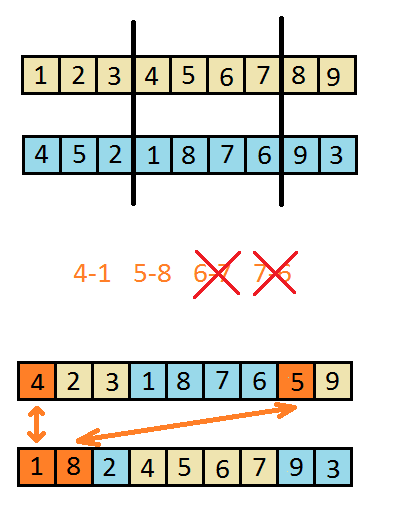
\includegraphics[scale=1]{pmx}
\caption{Krzyżowanie PMX}
\end{figure}

Podczas działania operatora OX, czyli operatora z zachowaniem porządku, wybierane są dwie pozycje genów z rozwiązań rodziców i spomiędzy tych pozycji kopiowane są geny z rodzica pierwszego do potomka pierwszego i z rodzica drugiego do potomka drugiego. Następnie, począwszy od pierwszej pozycji za kopiowanym fragmentem, przenoszone są geny z rodzica pierwszego do rozwiązania potomnego nr 2, z wyłączeniem elementów już się w nim znajdujących i na odwrót, czyli geny rodzica drugiego przenoszone są do potomka pierwszego. Przeniesione elementy są również umieszczane od pierwszej pozycji za skopiowanym fragmentem. Poniżej znajduje się rysunek obrazujący działanie tego operatora:

\newpage
\begin{figure}[h]
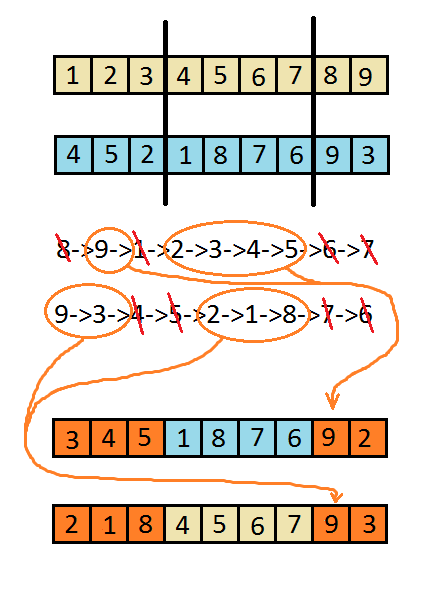
\includegraphics[scale=1]{ox}
\caption{Krzyżowanie OX}
\end{figure}

Zgodnie z założeniem autorów algorytmu, prawdopodobieństwo zajścia krzyżowania powinno zmniejszać się wraz z rosnącą liczbą iteracji algorytmu. W zmodyfikowanej wersji algorytmu możliwe jest ustawienie maksymalnego i minimalnego prawdopodobieństwa na tę samą wartość, co skutkuje niezmiennym prawdopodobieństwem krzyżowania podczas działania algorytmu.

Jeśli spośród wybranych na drodze działania operatora selekcji do krzyżowania zostanie przeznaczone mniej rozwiązań niż wynosi rozmiar populacji, z wybranych rozwiązań losowo kopiowane są brakujące osobniki i wstawiane są do listy przeznaczonych do krzyżowania rozwiązań w losowe miejsca. Następnie każde dwa kolejne rozwiązania na liście rodziców poddawane są wybranemu sposobowi krzyżowania i w ten sposób otrzymywane jest następne pokolenie rozwiązań, zastępujące poprzednie.

\subsection{Operator bramki kwantowej}
Oprócz przedstawionych wartości w tabeli \ref{LUT_TAB} zaproponowana została druga wersja tablicy \textit{Look Up}. Kąt zmieniany jest tylko w przypadku, gdy stany porównywanych kubitów są różne. W przypadku, gdy dopasowanie zapamiętanego rozwiązania najlepszego jest mniejsze niż poddawanego działaniu bramki kwantowej, zmiana kąta powoduje zwiększenie prawdopodobieństwa, że dany kubit pozostanie w swoim aktualnym stanie i wartość, o którą zmieniany jest kąt jest stosunkowo mała. W sytuacji, gdy dopasowanie rozwiązania najlepszego jest rzeczywiście lepsze, zmiana kąta następuje w kierunku zwiększenia prawdopodobieństwa, że kubit znajdzie się w stanie takim samym jak porównywany z nim odpowiadający mu kubit z rozwiązania najlepszego. W tym przypadku kąt jest zmieniany o wartość dużo większą niż w poprzedniej sytuacji. Zarówno jednak wartości, o które oba kąty są zmieniane, są dużo mniejsze niż wartości, które zostały zaproponowane w tabeli \ref{LUT_TAB}.

Poniżej znajduje się alternatywna wersja tablicy \textit{Look Up}:
\begin{table}[h]
\label{LUT_TAB_MOD}
\begin{tabular}{l l l l l l l l}
\hline
$r_i$ & $b_i$ & $f(r)<f(b)$ & $\Delta\Theta_i \cdot \pi$ & $s(\alpha_i,\beta_i)$ & & & \\
\cline{5-8} 
& & & & $\alpha_i \cdot \beta_i > 0$ & $\alpha_i \cdot \beta_i < 0$ & $\alpha_i = 0$ & $\beta_i = 0$ \\
\hline
0 & 1 & False & $0.08\pi$  & +1 & -1 & 0         & +1 lub -1\\
0 & 1 & True  & $0.001\pi$ & -1 & +1 & +1 lub -1 & 0\\
1 & 0 & False & $0.08\pi$  & -1 & +1 & +1 lub -1 & 0\\
1 & 0 & True  & $0.001\pi$ & +1 & -1 & 0         & +1 lub -1\\
\hline
\end{tabular}
\caption{Alternatywna LUT dla bramki kwantowej}
\end{table} 

W nieuwzględnionych przypadkach nie następuje aktualizacja kąta. Dotyczy to sytuacji, gdy zarówno kubit z rozwiązania najlepszego i aktualnie poddawanego działaniu bramki kwantowej, znajdują się w tym samym stanie, niezależnie od sytuacji, które z rozwiązań jest lepsze.

\subsection{Pozostałe zmiany}
W stosunku do algorytmu w postaci proponowanej w publikacji \cite{NPQGA}, wprowadzone zostały jeszcze dwie zmiany. Pierwszą z nich jest ustawianie wartości prawdopodobieństwa krzyżowania na wartość $P_{c min}$ w przypadku, gdy wyliczana w każdej iteracji jego wartość spadnie poniżej wartości $P_{c min}$. Druga modyfikacja związana jest z dekodowaniem stanów kubitów. Wedle autorów algorytmu, stan kubitu powinien być ustawiony na wartość 1, gdy wylosowany parametr $\eta$ jest mniejszy niż wartość $|\alpha|^2$, co nie jest prawdą, gdyż $|\alpha|^2$ określa prawdopodobieństwo, że kubit znajduje się w stanie 0.
\chapter{Aplikacja rozwiązująca problem przydziału kwadratowego z wykorzystaniem kwantowego algorytmu ewolucyjnego}
\label{cha:aplikacja}
Jednym z celów realizowanej pracy dyplomowej było napisanie aplikacji, która przy wykorzystaniu jednego z algorytmów aproksymacyjnych będzie rozwiązywać problem przydziału kwadratowego. Wybór padł na kwantowy algorytm ewolucyjny NPQGA opisany w rozdziale czwartym. Uwzględnione w nim zmiany oraz modyfikacje zostały przedstawione w piątym rozdziale. Program został zrealizowany jako aplikacja konsolowa i napisany w języku C\#. O tym, że aplikacja będzie konsolowa zadecydował fakt, iż jej celem nadrzędnym jest znajdywanie rozwiązania problemu QAP i ma służyć jako narzędzie pozwalające zweryfikować działanie algorytmu. Aspekty wizualne są jedynie dodatkiem, który nie wpływa na jakość rozwiązania problemu.

\section{Interfejsy klas}
Punktem wyjścia do rozpoczęcia prac był zestaw interfejsów klas przygotowanych przez opiekuna niniejszej pracy. Interfejs klasy w sensie języka C\# jest narzędziem wykorzystywanym w technice dziedziczenia i określa metody i właściwości, jakie klasa dziedzicząca po nim musi implementować. Jednakże ciała metod nie są określone i zależą wyłącznie od implementacji w danej klasie. W przeciwieństwie do dziedziczeniu po klasach, istnieje możliwość dziedziczenia po wielu interfejsach. Dzięki wykorzystaniu interfejsów, napisane na potrzeby pracy klasy będzie można wykorzystać w innych aplikacjach :już istniejących, ale i w tych, które dopiero powstaną. Poniżej znajduje się lista interfejsów, które należało zaimplementować:
\begin{enumerate}
\item IEvolutionAlgorithm,
\item IOptimisationAlgorithm,
\item IPopulation,
\item ISolution,
\item IEvolutionaryOperator,
\item IMutationOperator,
\item ICrossoverOperator.
\end{enumerate}

Interfejs \textit{IEvolutionAlgorithm} dziedziczy po interfejsie \textit{IOptimisationAlgorithm}. Na bazie tych interfejsów powstała klasa \textit{QgAlgorithm} zawierająca metody pozwalające na ustawienie i uruchomienie algorytmu oraz pozwalająca na zwrócenie rezultatów działania algorytmu.

Interfejsy \textit{ICrossoverOperator} i \textit{IMutationOperator} dziedziczące po interfejsie \textit{IEvolutionaryOperator} posłużyły jako podstawa, dla stworzenia klas realizujących zadania operatorów krzyżowania oraz mutacji. Na podstawie interfejsu \textit{ICrossoverOperator} powstała również klasa reprezentująca operator bramki kwantowej.

Interfejsy \textit{IPopulation} i \textit{ISolution} posłużyły do napisania klas reprezentujących odpowiednio pojedyncze rozwiązanie algorytmu i populację algorytmu.

\section{Struktura danych}
By algorytm mógł znaleźć rozwiązanie problemu, musi przetwarzać całą populację rozwiązań. Dlatego też została napisana klasa \textit{Population}, dziedzicząca po interfejsie \textit{IPopulation}. Populacja natomiast zawiera w sobie listę osobników, rozwiązań, które reprezentowane są przez obiekty klasy \textit{Solution} dziedziczącej z kolei po interfejsie \textit{ISolution}. Postacią rozwiązania w problemie przydziału kwadratowego jest permutacja, określająca, który obiekt został przypisany do kolejnych lokalizacji. Z tego powodu obiekty klasy \textit{Solution} zawierają w sobie listę obiektów reprezentujących elementy permutacji. Klasa tych obiektów została nazwana \textit{Chromosome}. Należy tutaj wyjaśnić pewną nieścisłość w terminach używanych w algorytmach genetycznych. \textit{Chromosomami} zwykło się nazywać kompletne rozwiązania, a ich fragmenty kodujące rozwiązanie \textit{genami}. Z racji, iż w aplikacji rozwiązania problemu reprezentowane są przez obiekty klasy \textit{Solution}, a element permutacji nie jest najmniejsza porcją informacji, postanowiono nazwać te porcje chromosomami, a ich najmniejszą część \textit{genem}. A więc \textit{chromosomy} składają się z kubitów reprezentowanych przez klasę \textit{Qbit}. Poprzez zdekodowanie stanu kubitów określa się wartość chromosomu, a następnie poprzez omówioną w rozdziale czwartym konwersję otrzymuje się permutacyjną postać rozwiązania problemu QAP.
\newpage
\begin{figure}[!t]
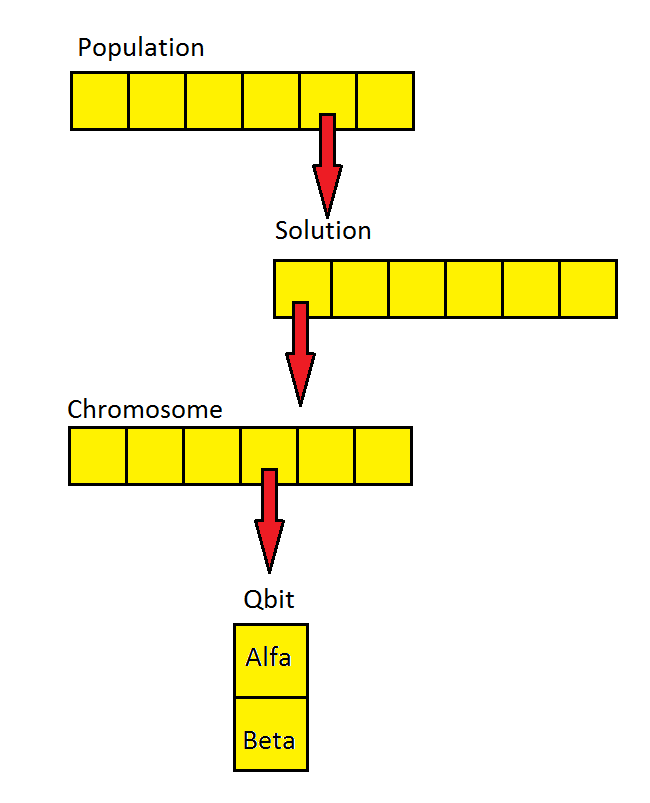
\includegraphics[scale=0.4]{data_structure}
\caption{Struktura danych}
\end{figure}

W kontekście struktury danych należy jeszcze wspomnieć o macierzach przepływu i odległości problemu QAP. Ich wartości są wczytywane z plików \textit{.dat} zawierających rozmiar problemu oraz odpowiednio macierze odległości i przepływu i są następnie trzymane w obiekcie klasy \textit{QapData} zrealizowanej jako singleton, czyli jako specjalna klasa o globalnym dostępnie pozwalająca na utworzenie tylko jednego jej obiektu. Posiada ona także mechanizmy, które bez wiedzy użytkownika same dbają o to, by faktycznie istniał jeden jej obiekt i jej instancja została utworzona podczas pierwszej próby jej użycia.

\section{Interfejs użytkownika}
Po uruchomieniu aplikacji użytkownik ma możliwość ustawienia kilku parametrów algorytmu. Należą do nich:
\begin{itemize}
\item wybór instancji problemu QAP,
\item rozmiar populacji, czyli ilość rozwiązań w populacji,
\item ilość iteracji algorytmu,
\item wybór sposobu selekcji rozwiązań,
\item wartość parametru $\eta_{max}$ w przypadku selekcji rankingowej,
\item minimalne i maksymalne prawdopodobieństwo krzyżowania,
\item operator krzyżowania,
\item prawdopodobieństwo mutacji,
\item wybór, czy stosować bramkę kwantową,
\item wersja bramki kwantowej,
\item wybór, czy otrzymane w wyniku działania algorytmu rezultaty i ustawione wartości parametrów zapisać do pliku,
\item nazwa pliku, do którego zostaną zapisane powyższe informacje.
\end{itemize}

W przypadku operatora selekcji do wyboru są dwie metody: ruletkowa oraz rankingowa. Spośród metod krzyżowania dostępne są trzy opcje: CX, OX i PMX. Wersje bramki kwantowej zostały opisane w rozdziałach 4 i 5.

Aplikacja została napisana w sposób niepozwalający na przyjęcie nieprawidłowych danych.

Po zakończeniu zwracane są rezultaty działania algorytmu i możliwe jest ponowne uruchomienie algorytmu. Użytkownik ma możliwość wyboru spośród trzech opcji:
\begin{enumerate}
\item ponowne uruchomienie dla tych samych parametrów i tej samej populacji początkowej,
\item ponowne uruchomienie dla tej samej populacji, lecz dla nowych wartości parametrów, z oczywistym pominięciem ustawiania rozmiaru populacji a także wyboru instancji testowej,
\item wygenerowanie nowej populacji i ustawienie nowych wartości parametrów.
\end{enumerate}

Opcja pierwsza pozwala sprawdzić różnice w otrzymanych rezultatach działania algorytmu przy tych samych parametrach. W tej sytuacji można sprawdzić, jaki wpływ na efekty końcowe ma czynnik losowy algorytmu.

Druga opcja pozwala na porównanie wpływu różnych wartości konkretnych parametrów na uzyskiwane rezultaty.

Opcja trzecia po prostu pozwala na ponowne uruchomienie algorytmu.

\section{Funkcja testująca parametry}
Oprócz opisanego wyżej interfejsu użytkownika została napisana również funkcja pozwalająca na przetestowanie zmieniającej się wartości wybranego parametru przy ustalonych pozostałych parametrach. Użytkownik podaje, który parametr chce przetestować, określa dla ilu jego wartości chce przeprowadzić testy oraz ile razy powtórzyć dany test, a także podaje, dla których instancji testowych przeprowadzić eksperymenty. Następnie należy określić wartości pozostałych parametrów, które będą stałe dla każdego z testów. Wymagane jest również podanie szablonu nazwy plików, w których zapisane są rezultaty eksperymentów. Cała nazwa pliku tworzona jest w następujący sposób sposób:
\newline
[szablon]\_[parametr testowany]\_[wartość parametru]\_[instancja testowa]\_[nr testu].

\section{Rezultaty działania aplikacji}
Po wykonaniu wszystkich iteracji algorytmu, program zwraca najlepsze znalezione rozwiązanie wraz z wartością funkcji celu oraz informację o tym, w której iteracji zostało zwrócone rozwiązanie. Zwracane jest również najlepsze rozwiązanie wraz z jego wartością funkcji celu uzyskane w ostatniej iteracji algorytmu.

Jeśli została wybrana opcja zapisu do pliku, tworzone są dwa pliki: w pierwszym z nich zapisane są ustawione parametry algorytmu wraz z datą uruchomienia algorytmu. W pliku zostaje też zawarta informacja o wartości najlepszego rozwiązania w ogóle wraz z numerem iteracji, w której zostało znalezione, a także jego postać. Podobnie, zawarta jest również informacja o najlepszym rozwiązaniu znalezionym w ostatniej iteracji. Drugi zawiera 3 kolumny danych zawierających odpowiednio numer iteracji, wartość najlepszego rozwiązania w danej iteracji i średnią wartość wszystkich rozwiązań w populacji. Zapis w tym formacie pozwala na późniejszy łatwy import danych do innych aplikacji pozwalających np. na utworzenie wykresów.

\section{Szczegóły związane z implementacją poszczególnych elementów algorytmu}
Kilka szczegółów związanych z działaniem algorytmu nie zostało poruszonych w publikacji \cite{NPQGA}. Jednakże , by algorytm mógł działać, należało arbitralnie przyjąć pewne założenia. Jednym z takich założeń jest moment aktualizacji stanu kubitów. Zostało przyjęte, że należy ocenić, w którym ze stanów 1 lub 0 znajduje się bit kwantowy, gdy wiadome jest, że rozwiązanie, w którym dany kubit się znajduje, poddane zostało zmianom wynikającym z działania operatora bramki kwantowej, lub dla tego rozwiązania zostały spełnione warunki na zajście mutacji. Natomiast po dokonaniu operacji krzyżowania, nie jest oceniany stan kubitów rozwiązań potomnych. Taka ocena, szczególnie w początkowych iteracjach algorytmu powodowałaby, że rozwiązania otrzymane na drodze krzyżowania mogłyby tracić informację uzyskaną z rozwiązań rodziców. Ideą krzyżowania jest wymiana informacji.

W przypadku, gdy użytkownik programu postanowi, że algorytm ma znajdywać rozwiązanie bez wykorzystania bramki kwantowej, kwantowa idea algorytmu przejawia się wtedy jedynie podczas tworzenia populacji początkowej oraz operacji mutacji, która dalej polega na zamianie wartości parametrów $\alpha$ i $\beta$.

Rozwiązanie, które jest podstawą do działania bramki kwantowej i nazywane jest najlepszym, jest faktycznie najlepszym rozwiązaniem, ale uzyskanym w poprzedniej iteracji. Operator bramki kwantowej używany jest dopiero na populacji poddanej już działaniu operatorów krzyżowania i mutacji. Z tego powodu istnieje możliwość, że dopasowanie zapamiętanego rozwiązania będzie gorsze niż dopasowanie niektórych rozwiązań poddawanych działaniu bramki kwantowej. Dlatego rozważane są w tablicach \textit{Look Up} przypadki, dla których warunek $f(x)>f(best)$ może być prawdą.

Foldery z rezultatami działania algorytmu - \textit{Results}i instancjami testowymi - \textit{QAPLib} znajdują się w tym samym folderze co plik wykonywalny aplikacji. Podczas tworzenia obiektu klasy \textit{QgAlgorithm} sprawdzane jest czy te foldery istnieją i jeśli nie, to są tworzone.

Próba przeprowadzenia testów, gdy folder z instancjami testowymi jest pusty, skutkuje zakończeniem działania funkcji interfejsu użytkownika i testującej parametry wraz z pojawieniem się na ekranie krótkiej informacji informującej, że folder jest pusty.
\chapter{Metodyka eksperymentów}
\label{cha:metodyka}

Możliwość ustawienia wielu różnych wartości parametrów zaimplementowanego w napisanej aplikacji algorytmu pozwala na przeprowadzenie serii eksperymentów badających ich wpływ na otrzymywane rezultaty. Również wprowadzenie wielu modyfikacji do samego algorytmu powoduje, że należy sprawdzić, czy te zmiany powodują istotne różnice w kwestii rozwiązywania problemu. Być może wprowadzone zmiany powodują, że algorytm znajduje rozwiązania niezgodne z oczekiwaniami, jego zbieżność uległa pogorszeniu. Z wymienionych przyczyn została przeprowadzona znaczna ilość testów z wykorzystaniem ogólnodostępnych instancji testowych weryfikujących poprawność ogólnego działania algorytmu oraz badających wpływ poszczególnych parametrów algorytmu na jego działanie.
 
\section{Instancje testowe}
\label{sec:instancje}
Popularność problemu QAP powoduje, że istnieje cała gama instancji testowych problemu z podanym optymalnym rozwiązaniem, lub najlepszym znalezionym rozwiązaniem dotychczas. Wykorzystane w eksperymentach instancje testowe pochodzą ze strony [adres] i są w postaci plików \textit{*.dat} zawierających rozmiar problemu i odpowiednio macierze odległości i przepływu. W przypadku, gdy jest inaczej, instancja opatrzona jest stosownym komentarzem. Podawane do instancji rozwiązania są permutacjami, których elementy reprezentują przydzielone obiekty, a pozycja w reprezentuje lokalizację.

Do testów zostały wybrane trzy konkretne instancje o różnym rozmiarze, wszystkie ze znanym optymalnym rozwiązaniem. Wybór instancji ze znanym rozwiązaniem podyktowany był tym, że znajomość optimum pozwala na lepszą analizę otrzymanych rezultatów oraz wybranych ustawień algorytmu.

Pierwszą wybraną instancją jest instancja \textit{Had12}. Jej autorami są S.W. Hadley, F. Rendl i H. Wolkowicz. Nazwa instancji pochodzi od nazwiska pierwszego z autorów i rozmiaru (12). Macierz odległości reprezentuje odległości pomiędzy połączonymi obiektami na Mahattanie, natomiast macierz przepływu jest wygenerowana na podstawie równomiernego rozkładu na przedziale \textit{[1,12]}. Znane jest optymalne rozwiązanie i jego wartość wynosi 1652, a jego postać wygląda w następujący sposób:
\newline
(3, 10, 11, 2, 12, 5, 6, 7, 8, 1, 4, 9).

Kolejną wybraną instancją jest problem o nazwie \textit{Lipa20a} autorstwa Y. Li i P.M. Pardalos. Podobnie jak powyżej, nazwa instancji pochodzi o jej rozmiaru i nazwisk autorów. Instancja ta nie ma konkretnego przełożenia na rzeczywistość, została wygenerowana w generatorze problemów. Optymalna wartość dla tego problemu to 3683, a postać rozwiązania jest następująca:
\newline
(19, 17, 7, 1, 5, 9, 10, 12, 4, 16, 20, 6, 3, 14, 11, 15, 13, 8, 2, 18).

Ostatnią, trzecią z wybranych instancji jest instancja \textit{Kra32}. Jej autorami są J. Krarup i P.M. Pruzan, a zawarte w niej dane są związane z rzeczywistymi danym wykorzystanymi podczas projektowania kliniki w Regensburgu w Niemczech. Optymalna wartość wynosi 88700, a postać rozwiązania optymalnego jest następująca:
\newline
(31, 23, 18, 21, 22, 19, 10, 11, 15, 9, 30, 29, 14, 12, 17, 26, 27, 28, 1, 7, 6, 25, 5, 3, 8, 24, 32, 13, 2, 20, 4, 16).    
 
\section{Scenariusze testowe}
\label{sec:scenariusze}
Z racji, iż stosunkowo duża ilość parametrów algorytmu może być zmieniana, nieraz w szerokim zakresie, nie jest możliwe przetestowanie wszystkich możliwych wariantów i porównania uzyskanych dla tych wariantów wyników. Dlatego skupiono się przede wszystkim na badaniu różnic w otrzymywanych rezultatach, gdy zmieniany był tylko jeden parametr. Poprzez wielokrotne uruchamianie algorytmu dla tej samej wygenerowanej populacji początkowej i dla tych samych parametrów uzyskiwane były uśrednione rezultaty. Algorytm z powodu swojej niedeterministycznej natury, zawierającej element losowości, nie pozwala na uzyskanie tych samych rezultatów przy tych samych ustawieniach przy wielokrotnym uruchamianiu. Dlatego więc uśrednianie wyników z wielu prób jest uzasadnione. W skrajnych przypadkach otrzymany wynik może informować o bardzo dobrym działaniu algorytmu, w innym o fatalnym. Algorytmy przybliżone stosowane są przede wszystkim tam, gdzie próby rozwiązania problemu metodami dokładnym z góry skazane są na niepowodzenie. W przeciwieństwie do eksperymentów, nie jest znane rozwiązanie problemu (gdyby było, jaki byłby cel stosowania tych algorytmów). Poszukiwanie rozwiązania jest wtedy procesem składającym się z wielu prób. Stosowana metodyka testów oddaje więc charakter faktycznych poszukiwań rozwiązania postawionego problemu. Analiza rezultatów eksperymentów pozwala na dobór odpowiednich ustawień parametrów algorytmu, przyczyniających się do efektywnego rozwiązywania problemów podobnych, dla których rozwiązanie nie jest znane. Każdy z opisanych niżej testów polegał na zmianie pewnego jednego testowanego parametru i powtarzany był dla każdej z instancji. Otrzymywane wyniki były porównywane ze sobą, z uwzględnieniem tego, dla której testowej instancji problemu były przeprowadzone. Uśrednione wyniki otrzymywane były na podstawie dziesięciu powtórzeń testu. Z racji iż, testowany algorytm w swoich założeniach wykorzystuje bramkę kwantową, poza pierwszą grupą testów, bramka ta zawsze była wykorzystywana, w wersji, która lepiej wypadła w pierwszym eksperymencie.

\subsection{Bramka kwantowa}
Jeszcze w trakcie pisania aplikacji, pojawiło się wiele wątpliwości związanych z operatorem bramki kwantowej. Idea jej stosowania wydaje się być wprawdzie słuszna - odpowiednia modyfikacja osobników w populacji zwiększająca ich prawdopodobieństwo na upodobnienie się ich do rozwiązania lepszego od nich i ,,utwierdzenia'' ich w swojej postaci, gdy są lepsze niż porównywane z nimi rozwiązanie gorsze. Jednakże, wykorzystanie jej w praktyce, w postaci proponowanej w publikacji [ref], często skutkuje otrzymywaniem rezultatów złych. Pojawiła się więc wątpliwość, czy na pewno operator ten jest dobry. Jego stosowanie wydaje się być jednak wymagane - poza mutacją, która teoretycznie zachodzi dość rzadko, operator ten ma możliwość na zmianę stanu bitów kwantowych, które są główną cechą algorytmów ewolucyjnych. Bez operatora bramki kwantowej algorytm staje się praktycznie typowym algorytmem genetycznym, w którym jego jedyny związek z kwantowym podejściem do problemu widoczny jest w operatorze mutacji. Z tego powodu została zaproponowana druga wersja bramki rotacyjnej, opisana w rozdziale 5. Seria eksperymentów związanych z wpływem bramki kwantowej na otrzymywane rezultaty miała więc na celu porównania trzech wariantów poszukiwania rozwiązania:
\begin{enumerate}
\item bez wykorzystania bramki kwantowej,
\item z wykorzystaniem bramki kwantowej w wersji proponowanej przez autorów algorytmu NPQGA,
\item z wykorzystaniem bramki kwantowej w wersji proponowanej przez autora niniejszej pracy. 
\end{enumerate}

\subsection{Operator selekcji}
Każda z dwóch zaimplementowanych metod selekcji ma swoje dobre i złe strony. Należało jednak sprawdzić, która z metod bardziej przydatna jest w przypadku postawionego problemu. Dodatkowo metoda rankingowa pozwala na ustawienie parametru $\eta$, dodatkowo więc należało sprawdzić wpływ tego parametru na uzyskiwane wyniki. Przeprowadzona została więc seria testów porównujących działania obu operatorów oraz seria eksperymentów porównujących działanie operatora selekcji rankingowej z różnymi wartościami parametru $\eta$: wartością minimalną, maksymalną i pośrednią. 

\subsection{Operator krzyżowania}
Każdy z trzech zaimplementowanych operatorów krzyżowania (CX, OX, PMX) ma inne działanie. W związku z tym krzyżowanie przeprowadzone przy wykorzystaniu jednego z operatorów powinno dać rezultaty inne niż dla innego operatora. Przebieg działania algorytmu genetycznego, uruchomionego dla tych samym parametrów przeważnie wygląda inaczej, nawet jeśli zwracane jest to samo rozwiązanie. W związku z tym, ciężko jest wprost porównać, który z operatorów krzyżowania działa lepiej lub gorzej. Jednakże w przypadku wielokrotnego powtórzenia tego samego testu z wykorzystaniem jednego operatora krzyżowania i uśrednienia wyników, może pozwolić na dostrzeżenie pewnych różnic pomiędzy rezultatami analogicznych testów z wykorzystaniem innego operatora. Z tego powodu testy dotyczące porównania działania operatorów krzyżowania polegały na wielokrotnym uruchamianiu algorytmu dla tych samych parametrów, populacji początkowej i z różnymi wybranymi operatorami krzyżowania.

\subsection{Prawdopodobieństwo krzyżowania}
Algorytm zaimplementowany w aplikacji pozwala na ustawienie minimalnego i maksymalnego prawdopodobieństwa krzyżowania. Ustawienie obu parametrów na tę samą wartość powoduje, że prawdopodobieństwo krzyżowania ma stała wartość podczas całego działania algorytmu. Należało więc sprawdzić jaki wpływ na otrzymywane rezultaty mają różne wartości stałego prawdopodobieństwa, a także czy zmieniająca się jego wartość w trakcie działania algorytmu powoduje istotne zmiany w efektywności poszukiwania optimum. Testy polegały więc, na porównaniu rezultatów otrzymanych dla małej, średniej i dużej wartości prawdopodobieństwa, a także na porównaniu wyników otrzymanych przy stałym i zmieniającym się prawdopodobieństwie krzyżowania. Przyjęto, że stała wartość prawdopodobieństwa jest średnią arytmetyczną wartości minimalnej i maksymalnej prawdopodobieństwa w teście ze zmiennym prawdopodobieństwem.

\subsection{Prawdopodobieństwo mutacji}
Przyjęło się mówić, że operator mutacji ma drugorzędne znaczenie w kwestii poszukiwania rozwiązań w algorytmie genetycznym. Jednakże natura tego operatora w kontekście zaimplementowanej wersji algorytmu może powodować znaczące zmiany w postaci mutowanego rozwiązania. Eksperymenty badające wpływ prawdopodobieństwa mutacji na otrzymywane rezultaty polegały na testowaniu trzech sytuacji:
\begin{enumerate}
\item prawdopodobieństwo mutacji równe 0,
\item wartość prawdopodobieństwa mała (w stosunku do prawdopodobieństwa krzyżowania),
\item wartość prawdopodobieństwa duża (rząd wielkości prawdopodobieństwa krzyżowania).
\end{enumerate}

\subsection{Najlepsze parametry}
Ostatni ze scenariuszy testowych jest niejako podsumowaniem scenariuszy wcześniejszych. Polegał on na poszukiwaniu rozwiązania problemu dla parametrów ustawionych na wartości, które na podstawie poprzednich testów uznane zostały za najlepsze (spośród wartości testowanych) i porównaniu otrzymanych wyników z wynikami uzyskanymi na podstawie działania algorytmu z ustawieniami najgorszymi. Test ten pozwala na sprawdzenie czy najlepsze znalezione w testach poprzednich wartości parametrów algorytmu ustawione razem również pozwalają na uzyskiwanie dobrych rozwiązań.

Rozdział ósmy poświęcony jest rezultatom uzyskanym w opisanych wyżej testach, a rozdział dziewiąty analizom uzyskanych w przeprowadzonych eksperymentach rezultatom. 
\chapter{Eksperymenty obliczeniowe}
\label{cha:eksperymenty}
\section{Bramka kwantowa}
W testach, których rezultaty znajdują się poniżej zmianie ulegała wersja bramki kwantowej, pozostałe parametry algorytmu były stałe i ich wartości znajdują się w tableli \ref{T1_params}:

\begin{table}[H]
\label{T1_params}
\begin{tabular}{l l l l l l l l}
\hline
liczba & rozmiar & min. prawd. & maks. prawd & operator & prawd. & selekcja & liczba \\
iteracji & populacji & krzyżowania & krzyżowania & krzyżowania & mutacji & & testów \\
\hline
300 & 50 & 0,8 & 0,8 & CX & 0,05 & ruletkowa & 5 \\
\hline
\end{tabular}
\caption{Stałe parametry eksperymentu związanego z bramka kwantową}
\end{table}

Poniżej znajdują się tabele z rezultatami otrzymany dla każdej z instancji testowej. Oznaczenia w pierwszym wierszu tabeli oznaczają odpowiednio: wartość funkcji celu najlepszego rozwiązania z populacji początkowej, wartość funkcji celu najlepszego z rozwiązań znalezionego w ogóle podczas wszystkich testów, średnią wartość funkcji celu dla najlepszych rozwiązań w każdym z testów, numer iteracji, w której znaleziono najlepsze rozwiązanie, średnią wartość numerów iteracji najlepszych rozwiązań w każdym z testów oraz błąd względny najlepszego z rozwiązań w stosunku do rozwiązania optymalnego.

\begin{table}[H]
\label{T1_bur26a}
\begin{tabular}{l l l l l l l}
\hline
 & $f_{init}$ & $f_{best}$ & $\overline{f_{best}}$ & n & $\overline{n}$ & $\delta$ \\
\hline
brak & 5684727 & 5571084 & 5576314,667 & 12 & 17,66666667 & 0,0266119 \\
oryginalna & 5684727 & 5531474 & 5552662,333 & 12 & 102,6666667 & 0,019312765 \\
zmodyfikowana & 5684727 & 5496454 & 5509412 & 116 & 171,3333333 & 0,012859452 \\
\hline
\end{tabular}
\caption{Rezultaty dla instancji bur26a}
\end{table}

\begin{table}[H]
\label{T1_chr15b}
\begin{tabular}{l l l l l l l}
\hline
 & $f_{init}$ & $f_{best}$ & $\overline{f_{best}}$ & n & $\overline{n}$ & $\delta$ \\
\hline
brak & 37898 & 24242 & 25478,66667 & 3 & 55 & 2,034042553\\
oryginalna & 37898 & 14828 & 16308 & 111 & 146,3333333 & 0,855819775\\
zmodyfikowana & 37898 & 15174 & 17303,33333 & 43 & 51 & 0,899123905\\
\hline
\end{tabular}
\caption{Rezultaty dla instancji chr15b}
\end{table}

\begin{table}[H]
\label{T1_chr18b}
\begin{tabular}{l l l l l l l}
\hline
 & $f_{init}$ & $f_{best}$ & $\overline{f_{best}}$ & n & $\overline{n}$ & $\delta$ \\
\hline
brak & 2950 & 2522 & 2671,333333 & 3 & 5,333333333 & 0,644067797\\
oryginalna & 2950 & 1882 & 1964 & 14 & 157 & 0,226857888\\
zmodyfikowana & 2950 & 1672 & 1777,333333 & 43 & 61,33333333 & 0,089960887\\
\hline
\end{tabular}
\caption{Rezultaty dla instancji chr18b}
\end{table}

\begin{table}[H]
\label{T1_chr25a}
\begin{tabular}{l l l l l l l}
\hline
 & $f_{init}$ & $f_{best}$ & $\overline{f_{best}}$ & n & $\overline{n}$ & $\delta$ \\
\hline
brak & 16356 & 11828 & 12355,33333 & 5 & 103,6666667 & 2,115911486\\
oryginalna & 16356 & 11054 & 11379,33333 & 114 & 162,6666667 & 1,912012645\\
zmodyfikowana & 16356 & 7716 & 8720,666667 & 75 & 95,66666667 & 1,032665964\\
\hline
\end{tabular}
\caption{Rezultaty dla instancji chr25a}
\end{table}

\begin{table}[H]
\label{T1_esc64a}
\begin{tabular}{l l l l l l l}
\hline
 & $f_{init}$ & $f_{best}$ & $\overline{f_{best}}$ & n & $\overline{n}$ & $\delta$ \\
\hline
brak & 228 & 148 & 173,3333333 & 15 & 17,66666667 & 0,275862069\\
oryginalna & 228 & 138 & 150,6666667 & 32 & 121,6666667 & 0,189655172\\
zmodyfikowana & 228 & 116 & 118,6666667 & 78 & 125,6666667 & 0\\
\hline
\end{tabular}
\caption{Rezultaty dla instancji esc64a}
\end{table}

\begin{table}[H]
\label{T1_had12}
\begin{tabular}{l l l l l l l}
\hline
 & $f_{init}$ & $f_{best}$ & $\overline{f_{best}}$ & n & $\overline{n}$ & $\delta$ \\
\hline
brak & 1768 & 1702 & 1724 & 1 & 6,333333333 & 0,030266344\\
oryginalna & 1768 & 1684 & 1688,666667 & 18 & 45 & 0,01937046\\
zmodyfikowana & 1768 & 1684 & 1700 & 28 & 35,33333333 & 0,01937046\\
\hline
\end{tabular}
\caption{Rezultaty dla instancji had12}
\end{table}

\begin{table}[H]
\label{T1_kra32}
\begin{tabular}{l l l l l l l}
\hline
 & $f_{init}$ & $f_{best}$ & $\overline{f_{best}}$ & n & $\overline{n}$ & $\delta$ \\
\hline
brak & 127190 & 113420 & 116506,6667 & 8 & 13,66666667 & 0,278692221\\
oryginalna & 127190 & 110950 & 112093,3333 & 96 & 211 & 0,250845547\\
zmodyfikowana & 127190 & 99100 & 102046,6667 & 112 & 180 & 0,117249154\\
\hline
\end{tabular}
\caption{Rezultaty dla instancji kra32}
\end{table}

\begin{table}[H]
\label{T1_lipa20a}
\begin{tabular}{l l l l l l l}
\hline
 & $f_{init}$ & $f_{best}$ & $\overline{f_{best}}$ & n & $\overline{n}$ & $\delta$ \\
\hline
brak & 3865 & 3853 & 3859,666667 & 0 & 3,666666667 & 0,046158023\\
oryginalna & 3865 & 3831 & 3840,333333 & 23 & 30,33333333 & 0,040184632\\
zmodyfikowana & 3865 & 3803 & 3819 & 43 & 62,66666667 & 0,032582134\\
\hline
\end{tabular}
\caption{Rezultaty dla instancji lipa20a}
\end{table}

\begin{table}[H]
\label{T1_lipa50b}
\begin{tabular}{l l l l l l l}
\hline
 & $f_{init}$ & $f_{best}$ & $\overline{f_{best}}$ & n & $\overline{n}$ & $\delta$ \\
\hline
brak & 1541214 & 1512985 & 1519929 & 19 & 63 & 0,25014873\\
oryginalna & 1541214 & 1510388 & 1512682,667 & 96 & 176,3333333 & 0,248002882\\
zmodyfikowana & 1541214 & 1486615 & 1490356,667 & 151 & 199 & 0,228359736\\
\hline
\end{tabular}
\caption{Rezultaty dla instancji lipa50b}
\end{table}

\begin{table}[H]
\label{T1_lipa80a}
\begin{tabular}{l l l l l l l}
\hline
 & $f_{init}$ & $f_{best}$ & $\overline{f_{best}}$ & n & $\overline{n}$ & $\delta$ \\
\hline
brak & 258029 & 257445 & 257612,6667 & 9 & 18,33333333 & 0,016785482\\
oryginalna & 258029 & 257363 & 257495,6667 & 34 & 180 & 0,01646162\\
zmodyfikowana & 258029 & 256700 & 256796 & 259 & 273,6666667 & 0,013843085\\
\hline
\end{tabular}
\caption{Rezultaty dla instancji lipa80a}
\end{table}

\begin{table}[H]
\label{T1_lipa90a}
\begin{tabular}{l l l l l l l}
\hline
 & $f_{init}$ & $f_{best}$ & $\overline{f_{best}}$ & n & $\overline{n}$ & $\delta$ \\
\hline
brak & 366925 & 366249 & 366354 & 21 & 23,33333333 & 0,015581066\\
oryginalna & 366925 & 366271 & 366355,6667 & 50 & 140,6666667 & 0,015642071\\
zmodyfikowana & 366925 & 365195 & 365309,6667 & 266 & 280,6666667 & 0,012658403\\
\hline
\end{tabular}
\caption{Rezultaty dla instancji lipa90a}
\end{table}

\section{Operator krzyżowania}
W eksperymencie dotyczącym operatora krzyżowania porównywane były rezultaty otrzymane przy użyciu różnych operatorów krzyżowania. Niezmienne parametry algorytmu ustawione były na te same wartości przedstawione w poniższej tabeli:

\begin{table}[H]
\label{T2_params}
\begin{tabular}{l l l l l l l l}
\hline
liczba & rozmiar & min. prawd. & maks. prawd & bramka & prawd. & selekcja & liczba \\
iteracji & populacji & krzyżowania & krzyżowania & kwantowa & mutacji & & testów \\
\hline
300 & 50 & 0,8 & 0,8 & zmodyfikowana & 0,05 & ruletkowa & 5 \\
\hline
\end{tabular}
\caption{Stałe parametry eksperymentu związanego z operatorem krzyżowania}
\end{table}

W poniższych tabelach znajdują się rezultaty testów dla poszczególnych instancji testowych:

\begin{table}[H]
\label{T2_bur26a}
\begin{tabular}{l l l l l l l}
\hline
 & $f_{init}$ & $f_{best}$ & $\overline{f_{best}}$ & n & $\overline{n}$ & $\delta$ \\
\hline
CX & 5717454 & 5509912 & 5512025,667 & 63 & 184,6666667 & 0,015339425\\
OX & 5717454 & 5545330 & 5575050 & 9 & 158 & 0,02186608\\
PMX	& 5717454 & 5499264 & 5536580,333 & 95 & 183,6666667 & 0,013377265\\
\hline
\end{tabular}
\caption{Rezultaty dla instancji bur26a}
\end{table}

\begin{table}[H]
\label{T2_chr15b}
\begin{tabular}{l l l l l l l}
\hline
 & $f_{init}$ & $f_{best}$ & $\overline{f_{best}}$ & n & $\overline{n}$ & $\delta$ \\
\hline
CX & 31212 & 17554 & 18410,66667 & 55 & 100 & 1,196996245\\
OX & 31212 & 17304 & 20116,66667 & 66 & 148,3333333 & 1,165707134\\
PMX & 31212 & 19892 & 21148 & 118 & 175,6666667 & 1,489612015\\
\hline
\end{tabular}
\caption{Rezultaty dla instancji chr15b}
\end{table}

\begin{table}[H]
\label{T2_chr18b}
\begin{tabular}{l l l l l l l}
\hline
 & $f_{init}$ & $f_{best}$ & $\overline{f_{best}}$ & n & $\overline{n}$ & $\delta$ \\
\hline
CX & 3550 & 1808 & 1865,333333 & 59 & 108,3333333 & 0,178617992\\
OX & 3550 & 2216 & 2262 & 53 & 117,6666667 & 0,444589309\\
PMX & 3550 & 1668 & 1840,666667 & 231 & 263,6666667 & 0,087353325\\
\hline
\end{tabular}
\caption{Rezultaty dla instancji chr18b}
\end{table}

\begin{table}[H]
\label{T2_chr25a}
\begin{tabular}{l l l l l l l}
\hline
 & $f_{init}$ & $f_{best}$ & $\overline{f_{best}}$ & n & $\overline{n}$ & $\delta$ \\
\hline
CX & 14380 & 9124 & 9658,666667 & 84 & 102 & 1,403582719\\
OX & 14380 & 11790 & 12020 & 151 & 208 & 2,105900948\\
PMX & 14380 & 11288 & 11499,33333 & 43 & 68,66666667 & 1,973656481\\
\hline
\end{tabular}
\caption{Rezultaty dla instancji chr25a}
\end{table}

\begin{table}[H]
\label{T2_esc64a}
\begin{tabular}{l l l l l l l}
\hline
 & $f_{init}$ & $f_{best}$ & $\overline{f_{best}}$ & n & $\overline{n}$ & $\delta$ \\
\hline
CX & 244 & 124 & 126 & 119 & 155 & 0,068965517\\
OX & 244 & 186 & 192 & 30 & 128 & 0,603448276\\
PMX & 244 & 162 & 164,6666667 & 58 & 186,3333333 & 0,396551724\\
\hline
\end{tabular}
\caption{Rezultaty dla instancji esc64a}
\end{table}

\begin{table}[H]
\label{T2_had12}
\begin{tabular}{l l l l l l l}
\hline
 & $f_{init}$ & $f_{best}$ & $\overline{f_{best}}$ & n & $\overline{n}$ & $\delta$ \\
\hline
CX & 1812 & 1678 & 1685,333333 & 32 & 43,33333333 & 0,015738499\\
OX & 1812 & 1686 & 1690,666667 & 30 & 118,6666667 & 0,020581114\\
PMX	& 1812 & 1690 & 1693,333333 & 69 & 150,6666667 & 0,023002421\\
\hline
\end{tabular}
\caption{Rezultaty dla instancji had12}
\end{table}

\begin{table}[H]
\label{T1_kra32}
\begin{tabular}{l l l l l l l}
\hline
 & $f_{init}$ & $f_{best}$ & $\overline{f_{best}}$ & n & $\overline{n}$ & $\delta$ \\
\hline
CX & 126660 & 96620 & 97800 & 109 & 209 & 0,089289741\\
OX & 126660 & 114210 & 116090 & 99 & 167 & 0,287598647\\
PMX & 126660 & 111780 & 112970 & 258 & 274,3333333 & 0,260202931\\
\hline
\end{tabular}
\caption{Rezultaty dla instancji kra32}
\end{table}

\begin{table}[H]
\label{T2_lipa20a}
\begin{tabular}{l l l l l l l}
\hline
 & $f_{init}$ & $f_{best}$ & $\overline{f_{best}}$ & n & $\overline{n}$ & $\delta$ \\
\hline
CX & 3877 & 3831 & 3843 & 48 & 72 & 0,040184632\\
OX & 3877 & 3841 & 3847 & 75 & 143,6666667 & 0,04289981\\
PMX & 3877 & 3844 & 3845 & 38 & 51,33333333 & 0,043714363\\
\hline
\end{tabular}
\caption{Rezultaty dla instancji lipa20a}
\end{table}

\begin{table}[H]
\label{T2_lipa50b}
\begin{tabular}{l l l l l l l}
\hline
 & $f_{init}$ & $f_{best}$ & $\overline{f_{best}}$ & n & $\overline{n}$ & $\delta$ \\
\hline
CX & 1543705 & 1487038 & 1493044,333 & 212 & 257 & 0,228709252\\
OX & 1543705 & 1520666 & 1522054,333 & 20 & 52 & 0,256495384\\
PMX & 1543705 & 1519178 & 1520194,667 & 16 & 122 & 0,25526588\\
\hline
\end{tabular}
\caption{Rezultaty dla instancji lipa50b}
\end{table}

\begin{table}[H]
\label{T2_lipa80a}
\begin{tabular}{l l l l l l l}
\hline
 & $f_{init}$ & $f_{best}$ & $\overline{f_{best}}$ & n & $\overline{n}$ & $\delta$ \\
\hline
CX & 258140 & 256810 & 256962,3333 & 256 & 277 & 0,014277533\\
OX & 258140 & 257752 & 257764,3333 & 180 & 211 & 0,017997986\\
PMX & 258140 & 257697 & 257705,6667 & 67 & 167 & 0,017780762\\
\hline
\end{tabular}
\caption{Rezultaty dla instancji lipa80a}
\end{table}

\begin{table}[H]
\label{T2_lipa90a}
\begin{tabular}{l l l l l l l}
\hline
 & $f_{init}$ & $f_{best}$ & $\overline{f_{best}}$ & n & $\overline{n}$ & $\delta$ \\
\hline
CX & 366995 & 365281 & 365551,6667 & 278 & 288 & 0,012896875\\
OX & 366995 & 366456 & 366485,3333 & 7 & 191,6666667 & 0,016155062\\
PMX	& 366995 & 366474 & 366554,3333 & 31 & 167,6666667 & 0,016204975\\
\hline
\end{tabular}
\caption{Rezultaty dla instancji lipa90a}
\end{table}

\chapter{Analiza uzyskanych wyników}
\label{cha:analiza}

Stwierdzenie, która wartość wybranego parametru algorytmu jest lepsza, jest zadaniem trudnym. Przyjęto więc, że w pierwszej kolejności decyzję należy podjąć w oparciu o wartość błędu względnego, a w przypadku gdy różnice są niewielkie, wybór najlepszej wartości testowanego parametru podejmowany jest na podstawie średniej wartości numerów iteracji algorytmu, w których uzyskano najlepsze rozwiązania.

Należy oczywiście podkreślić, iż stwierdzenie, że wybrana wartość parametru jest najlepsza, dotyczy tylko wartości testowanych. Nie jest wiadome, czy inna wartość, która nie była sprawdzana eksperymentalnie nie pozwoliłaby na uzyskanie lepszych rezultatów. Natomiast wartości te starano się dobrać w taki sposób, by można było odpowiedzieć na pytanie, czy, przykładowo, testowany parametr powinien przyjmować wartości większe czy mniejsze.

Można zauważyć, że dla pewnych instancji testowych wartości błędów względnych są duże i nie ma znaczenia, który parametr algorytmu był testowany. Sytuacja ta może wynikać z wielu powodów. Przyczyną niewątpliwie może być zły dobór parametrów, które nie podlegały aktualnie testowaniu. Być może dla jednej konkretnej instancji, dużo lepiej spisywałby się inny operator krzyżowania, pod warunkiem, że prawdopodobieństwo mutacji było inne. Być może instancja problemu skonstruowana jest tak, by istniało wiele minimów lokalnych o podobnej postaci do rozwiązania optymalnego.

\section{Bramka kwantowa}
Testowane były trzy warianty: brak bramki kwantowej, wersja bramki zaproponowana w \cite{NPQGA} oraz wersja nazywana zmodyfikowaną, zaproponowana przez autora niniejszej pracy. Poniżej znajduje się tabela zawierająca informację na temat, ile razy dany wariant pozwolił na uzyskanie lepszych rezultatów:

\begin{table}[H]
\label{bramka_results}
\begin{center}
\begin{tabular}{l l l}
\hline
brak bramki & wersja oryginalna & wersja zmodyfikowana \\
\hline
0 & 0 & 11\\
\hline
\end{tabular}
\end{center}
\caption{Porównanie wersji bramki kwantowej}
\end{table}

Powyższa tabela jednoznacznie pokazuje, przy opisanych wyżej kryteriach oceny, która ,,wartość'' bramki kwantowej jest najlepsza. Jednakże, dla niektórych instancji testowych różnice bywały niewielkie. 

Przy analizie jedynie średniej wartości numerów iteracji, zauważyć można, że wartość była najmniejsza dla sytuacji, gdy bramka kwantowa w ogóle była niewykorzystywana, a największa dla wersji zmodyfikowanej. Świadczy to o tym, że bramka ta pozwala unikać zbyt szybkiej zbieżności do minimum lokalnego. Natomiast różnice na korzyść wersji zmodyfikowanej można tłumaczyć tym, że sposób jej działania ma lepszy wpływ na szersze przeszukiwanie przestrzeni rozwiązań - nakierowuje ona przetwarzane rozwiązania na rozwiązanie lepsze od nich, lecz w przeciwieństwie do wersji oryginalnej zmiana kąta jest dużo mniejsza. Dzięki temu ewentualna zbieżność do minimum lokalnego jest mniej prawdopodobna.

Należy też wspomnieć, że publikacja \cite{NPQGA} zawierała opis algorytmu i jego wykorzystanie w problemie szeregowania zadań. W eksperymentach użyty algorytm był po wielu modyfikacjach względem swojej oryginalnej wersji i posłużył do rozwiązywania innego problemu. Być może to również miało wpływ na efekty uzyskiwane przy wykorzystani oryginalnej wersji bramki kwantowej. Możliwe jest, że wartości w tablicy \textit{Look Up} dobrane były specjalnie pod kątem problemu szeregowania zadań i dla innych problemów wartości te niekoniecznie muszą być odpowiednie.

Dla jednej instancji - \textit{esc64a} korzystając z bramki w wersji zmodyfikowanej udało się uzyskać rozwiązanie równe optymalnemu, gdzie średnia wartość numerów iteracji wynosiła około 126, a dla wersji oryginalnej przy wartości błędu około 0,19 średnia wartości iteracji wynosiła mniej więcej 122.

\section{Operator krzyżowania}
Kolejnym, drugim testowanym parametrem był operator krzyżowania. Testowane były operatory CX, OX oraz PMX. W poniższej tabeli znajduje się podsumowanie, ile razy dany operator okazał się najlepszy:

\begin{table}[H]
\label{cross_oper_results}
\begin{center}
\begin{tabular}{l l l}
\hline
CX & OX & PMX \\
\hline
8 & 1 & 2\\
\hline
\end{tabular}
\end{center}
\caption{Porównanie operatorów krzyżowania}
\end{table}

Z powyższej tabeli wynika, że najlepszym operatorem okazał się operator CX, jednakże nie było tak w każdym przypadku. Dla instancji \textit{chr15b} lepszy okazał się operator OX, natomiast dla instancji \textit{bur26a} i \textit{chr18b} PMX.

W przypadku operatorów krzyżowania trudno ocenić, dlaczego jeden działa lepiej od innych. Sam proces krzyżowania w problemie, którego rozwiązaniem jest permutacja, powoduje duże zmiany w rozwiązaniach potomnych. Oczywiście rozwiązania te mają cechy swoich rodziców, lecz sposób, w jaki informacja jest wymieniana, wprowadza duże modyfikacje. W permutacji ważna jest kolejność jej elementów, natomiast krzyżowanie nierzadko kolejność tę zaburza. Z tego wynika być może, że operator CX w mniejszym stopniu powoduje te modyfikacje.

W żadnym z przypadków nie udało się uzyskać rozwiązania optymalnego, choć często błąd względny był niewielki. Natomiast w przypadku instancji \textit{chr25a} dla każdego z operatorów wartość błędu wynosiła grubo ponad 1, a dla operatora OX nawet ponad 2.

\section{Prawdopodobieństwo krzyżowania}
Algorytm NPQGA w swych założeniach pozwala na zmianę wartości krzyżowania w czasie. Wartość ta wraz z rosnącą liczbą wykonanych iteracji algorytmu malała do określonej wartości minimalnej, by osiągnąwszy ją nie zmieniać się już do końca działania algorytmu. Testy dotyczące wpływu prawdopodobieństwa krzyżowania na otrzymywane rezultaty miały na celu pokazanie, czy zmieniająca się jego wartość ma realny wpływ na rezultaty i jaka jego wartość jest najlepsza. Poniższa tabela pokazuje, ile razy dla jakiej wartości prawdopodobieństwa uzyskano najlepsze rezultaty (podane są odpowiednio wartości minimalne i maksymalne prawdopodobieństwa krzyżowania):

\begin{table}[H]
\label{cross_prob_results}
\begin{center}
\begin{tabular}{l l l l l l}
\hline
0,8/0,8 & 0,6/1 & 0,6/0,6 & 0,4/0,8 & 0,4/0,4 & 0,2/0,6\\
\hline
1 & 4 & 2 & 0 & 3 & 1\\
\hline
\end{tabular}
\end{center}
\caption{Porównanie wartości prawdopodobieństwa krzyżowania}
\end{table}

Z powyższej tabeli wynika wprawdzie jednoznacznie, która wartość prawdopodobieństwa jest lepsza od innych, nie wynika jednak z niej, która wartość jest wyraźnie lepsza od innych. Sytuacja ta wydaje się być ciekawa - krzyżowanie jest zasadniczą częścią algorytmów genetycznych, a więc dobór właściwej wartości jego prawdopodobieństwa powinien być rzeczą bardzo ważną. Być może obecność bramki kwantowej powoduje to, że krzyżowanie traci na znaczeniu - nie jest już jedynym operatorem polepszającym wartość populacji z pokolenia na pokolenie.

Analizując tabelę \ref{cross_prob_results} można dojść do wniosku, że najlepsze rezultaty pozwoli osiągnąć prawdopodobieństwo krzyżowania o wartości równiej mniej więcej 0,6. Warto jednak przy tym podkreślić, że różnice pomiędzy błędami względnymi wyliczonymi dla każdej sytuacji nie są duże.

\section{Prawdopodobieństwo mutacji}
Niewątpliwie, sposób w jaki przeprowadzana jest mutacja w algorytmie NPQGA powoduje, że jej wpływ na rozwiązania, które zostały jej poddane jest dużo większy niż w innych algorytmach genetycznych.

Poniższa tabela prezentuje, ile razy testowana wartość prawdopodobieństwa mutacji pozwoliła na uzyskanie lepszych rezultatów niż pozostałe:

\begin{table}[H]
\label{bramka_results}
\begin{center}
\begin{tabular}{l l l}
\hline
0,4 & 0,05 & 0 \\
\hline
5 & 3 & 3 \\
\hline
\end{tabular}
\end{center}
\caption{Porównanie wartości prawdopodobieństwa mutacji}
\end{table}

Podsumowanie wyników przedstawione w powyższej tabeli może wydawać się lekko zaskakujące. Lepsze rezultaty uzyskano przeważnie w sytuacji, gdy wartość prawdopodobieństwa mutacji wynosiła 0,4. Wynikać z tego może fakt, że częstsza mutacja zwiększa prawdopodobieństwo zdekodowania rozwiązania w taki sposób, że jest ono bardziej podobne do rozwiązania lepszego, uwzględnianego w działaniu bramki kwantowej. Równocześnie, małe różnice w uzyskiwanych rezultatach dla wszystkich testowanych wartości prawdopodobieństwa mutacji mogą potwierdzać tezę, że mutacja ma dużo mniejszy wpływ na osiągane przez algorytm wyniki niż operacja krzyżowania.

Dla instancji testowej o nazwie \textit{chr15b} uzyskany błąd względny dla każdego przypadku był duży, a dla wartości prawdopodobieństwa mutacji równego 0,4 osiągnął wartość przekraczającą 1. Udało się także raz znaleźć rozwiązanie optymalne. Sytuacja ta miała miejsce dla instancji \textit{esc64a} i wartości prawdopodobieństwa mutacji równego 0,05.

\section{Operator selekcji}
Ostatnim testowanym parametrem algorytmu był operator selekcji. Testom podlegała selekcja ruletkowa oraz rankingowa dla różnych wartości parametru $\eta$. Poniższa tabela przedstawia, ile razy dany z wariantów okazał się lepszy od pozostałych:

\begin{table}[H]
\label{bramka_results}
\begin{center}
\begin{tabular}{l l l l}
\hline
selekcja & selekcja & selekcja & selekcja\\
ruletkowa & rankingowa, $\eta = 1$ & rankingowa, $\eta = 1,5$ & rankingowa, $\eta = 2$\\
\hline
2 & 2 & 2 & 5\\
\hline
\end{tabular}
\end{center}
\caption{Porównanie operatorów selekcji}
\end{table}

Z poniższej tabeli wynika, że najczęściej najlepsze rezultaty uzyskano, gdy wybrana była selekcja rankingowa, z parametrem $\eta$ równym 2, czyli dla wartości największej możliwej i najbardziej premiującej rozwiązania lepsze od gorszych. Co ciekawe, dla dwóch instancji testowych  mimo ustawienia parametru $\eta$ na wartość 1 udało się uzyskać lepsze rezultaty niż dla wartości innych. W takim przypadku rozwiązania są wybierane losowo, gdyż każde z nich ma takie same prawdopodobieństwo bycia wybranym. Sytuacja ta mogła być wynikiem tego, że przy danym rozmiarze populacji różnice w prawdopodobieństwach wyboru rozwiązań dla parametru $\eta$ różnego od 1 i dla selekcji ruletkowej są małe i rozwiązanie najgorsze w pokoleniu ma niewiele mniejszą szansę bycia wybranym niż najlepsze. Z tego powodu selekcja w każdym z możliwych przypadków przebiega dość podobnie.

\section{Najlepsze parametry}
Ostatni podsumowujący eksperyment miał na celu zweryfikowanie, czy uzyskane najlepsze wartości parametrów w każdym z wcześniejszych testów, ustawione razem poprawią uzyskiwane rezultaty. Poniższa tabela zawiera informacje na temat tego, ile razy dla danej instancji testowej udało się uzyskać poprawę, a ile razy wynik był gorszy w stosunku do poprzednich eksperymentów:
\begin{table}[H]
\label{best_porownanie}
\begin{center}
\begin{tabular}{l l l}
\hline
instancja testowa & ile razy lepszy wynik & ile razy gorszy wynik\\
\hline
bur26a & 4 & 1\\
chr15b & 2 & 3\\
chr18b & 2 & 3\\
chr25a & 1 & 4\\
esc64a & 4 & 1\\
had12 & 5 & 0\\
kra32 & 0 & 5\\
lipa20a & 3 & 2\\
lipa50b & 0 & 5\\
lipa80a & 1 & 4\\
lipa90a & 2 & 3\\
\hline
$\Sigma$ & 24 & 31\\
\hline
\end{tabular}
\end{center}
\caption{Porównanie wyników eksperymentów}
\end{table}

Powyższa tabela nie pozwala stwierdzić, że ustawienie parametrów na wartości uznane w poprzednich eksperymentach za najlepsze, spowodowało ogólne polepszenie działania algorytmu. Jednakże nie pozwala ona również stwierdzić, że taki dobór parametrów spowodował pogorszenie wyników. Zaistniała sytuacja może mieć swoją przyczynę w tym, że pewne parametry dobrane razem dadzą gorsze wyniki niż, gdyby każdy z nich był ustawiony na swoją teoretycznie najlepszą wartość w osobnych testach. Należy jednak wspomnieć, że różnice pomiędzy wcześniejszymi testami a testem ,,podsumowującym'' były niewielkie.

\section{Podsumowanie eksperymentów obliczeniowych}
Przeprowadzone eksperymenty przy użyciu napisanej aplikacji zweryfikowały poprawności jej działania - algorytm działa poprawnie, w większości przypadków otrzymane rezultaty były dość dobre. Jeden z testów pozwolił nawet na znalezienie rozwiązania optymalnego. Jednakże dla pewnych instancji testowych otrzymywane wyniki były złe, niezależnie od dobranych parametrów algorytmu. 

Niewielkie różnice pomiędzy uzyskiwanymi rezultatami eksperymentów pozwalają stwierdzić, że choć istnieją różne wersje operatorów genetycznych, każda z nich pozwala na uzyskiwanie dobrych rezultatów. Liczba parametrów algorytmu, które można zmienić oraz ich zakres, nie pozwolił na przetestowanie każdej możliwej opcji, dlatego należy jeszcze raz podkreślić, że wartości uznane za najlepsze, najlepszymi były tylko w obrębie danego eksperymentu, co niejako potwierdza eksperyment podsumowujący. Jednak rezultaty testów pozwalają na wyrobienie pewnej intuicji, dzięki której możliwy będzie właściwy dobór parametrów w przypadku rozwiązywania problemów, dla których nieznane jest rozwiązanie optymalne.  
\chapter{Analiza uzyskanych wyników}
\label{cha:analiza}
\chapter{Podsumowanie i wnioski}
\label{cha:wnioski}

Algorytmy przybliżone są potężnym narzędziem do rozwiązywania problemów, dla których algorytmy dokładne nie miałby możliwości na osiągnięcie sukcesu.

Operator mutacji w postaci wykorzystanej w algorytmie NPQGA może powodować duże zmiany w postaci rozwiązania dla którego zaszła mutacja

Kwantowa idea algorytmu może powodować, że mimo dużego prawdopodobieństwa na znalezienie się w danym stanie, kubit może znaleźć się w stanie przeciwnym. Może to powodować znaczne pogorszenie rozwiązania.
\bibliographystyle{alpha}
%\bibliography{bibliografia}
\begin{thebibliography}{99}

\bibitem{ANT_DISC} Dorigo, Marco, Di Caro, Gambardella, Gianni, Luca M. \textit{Ant Algorithms for Discrete Optimization}.

\bibitem{FIL_ROJOWE} Filipowicz Bogusław, Chmiel Wojciech, Kadłuczka Piotr, \textit{Ukierunkowane poszukiwanie przestrzeni rozwiązań w algorytmach rojowych}, Półrocznik Automatyka, z. 2m t. 13, Wydawnictwo AGH, Kraków 2009.

\bibitem{FILIP_STADNE} Filipowicz Bogusław, Kwiecień Joanna, \textit{Algorytmy stadne w optymalizacji problemów przydziału przy kwadratowym wskaźniku jakości (QAP)}, Półrocznik Automatyka, z. 2, t. 15, Wydawnictwo AGH, Kraków 2011.

\bibitem{TABU} Glover Fred, \textit{Tabu Search: A Tutorial}.

\bibitem{TABU_P1} Glover Fred, \textit{Tabu Search - Part I}, ORSA Journal on Computing, nr 3, t. 1, 1989.

\bibitem{GOLDBERG} Goldberg David E., \textit{Algorytmy genetyczne i ich zastosowania}, przeł. Kazimierz Grygiel, Wyd 3, Wydawnictwa Naukowo - Techniczne, Warszawa 2003.

\bibitem{NPQGA} Gu Jinwei, Gu Xingsheng, Gu Manzhan, \textit{A novel parallel quantum genetic algorithm for stochastic job shop scheduling}, Journal of Mathematical Analysis and Applications, 63-81, 2009.

\bibitem{AE_GWIAZDA} Gwiazda Tomasz Dominik, \textit{ ewolucyjne w rozwiązywaniu nieliniowych problemów decyzyjnych}, Wydawnictwa Naukowe Wydziału Zarządzania Uniwersytetu Warszawskiego, Warszawa 2002.

\bibitem{INTRO} Hiller Frederick S., Lieberman Gerald J., \textit{Introduction to Operations Research}, Wyd 5, McGraw - Hill Publishing Company, Nowy Jork 1990.

\bibitem{APROX_JONES} Jones Gareth, \textit{Genetic and Evolutionary Algorithms}, 1990.

\bibitem{QAP_DEF_CHMIEL} Kadłuczka Piotr, Chmiel Wojciech, \textit{Efektywność algorytmu ewolucyjnego wykorzystującego warunkową wartość oczekiwaną funkcji celu}, Półrocznik Automatyka, z. 1-2, t. 9, Wydawnictwo AGH, Kraków 2005.

\bibitem{PSO} Kennedy James, Eberhart Russel, \textit{Particle Swarm Optimization}, Materiały IEEE International Conference on Neural Networks, 4, 1942-1948, 1995.

\bibitem{SWARM_INT} Kennedy James, Eberhart Russel C., \textit{Swarm Intelligence}, Morgan Kaufmann Publishers, San Francisco, 2001.

\bibitem{COMPARISON} Laboudi Zakaria, Chikhi Salim,  \textit{Comparison of Genetic Algorithm and Quantum
Genetic Algorithm}, The International Arab Journal of Information Technology, nr 3, t. 9, 2012.

\bibitem{PSO2} Liu Hongbo, Abraham Ajith, Zhang Jianying \textit{A Particle Swarm Approach to Quadratic Assignment Problems}. [w:] Soft Computing in Industrial Applications, pod red. Saad A., Dahal K., Sarfraz M., Roy R., Springer, Berlin 2007.

\bibitem{MICH_AG} Michalewicz Zbigniew, \textit{Algorytmy genetyczne + struktury danych = programy ewolucyjne}, przeł. Zbigniew Nahorski, Wyd 3, Wydawnictwa Naukowo-  Techniczne, Warszawa 2003.

\bibitem{MICH_JAK} Michalewicz Zbigniew, Fogel David B., \textit{jak to rozwiązać czyli nowoczesna metaheurystyka}, przeł. Aleksy Schubert, Joanna Schubert, Wydawnictwa Naukowo - Techniczne, Warszawa 2006.

\bibitem{META_HEU} Stawowy Adam, \textit{Heurystyki i metaheurystyki}, wykład z przedmiotu Inteligencja Obliczeniowa.

\bibitem{ACO_DORIGO} St\"utzle Thomas, Dorigo Marco, \textit{ACO Algorithms for the Quadratic Assignment Problem}. [w:] D. Corne, M. Dorigo, F. Glover, New Ideas for Optimization, McGraw-Hill, 1999, 33-50.

\bibitem{APROX} Vizirani Vijay V., \textit{Approximation Algorithms}, Springer, Berlin 2003.

\bibitem{INSTANCJE} Zbiór instancji testowych problemu QAP: http://anjos.mgi.polymtl.ca/qaplib/inst.html.

\end{thebibliography}
\chapter*{DODATEK A}
\addcontentsline{toc}{chapter}{DODATEK A}
\chapter*{DODATEK B}
\addcontentsline{toc}{chapter}{DODATEK B}
\end{document}
